\documentclass[a4paper,11pt,nocenter,bold,notitlepage,noheadline,noindent]{thesis}

\usepackage[latin1]{inputenc}
\usepackage{amsmath}
\usepackage{amsfonts}
\usepackage{amssymb}
\usepackage{graphicx}
\usepackage{textcomp}
\usepackage{url}
\usepackage{graphicx}
\usepackage[numbers]{natbib}
\usepackage{caption}
\usepackage{subcaption}
\usepackage{pdfpages}
\usepackage{booktabs}
\usepackage{pdflscape}
\usepackage{listings}
\lstset{%
	basicstyle=\ttfamily,
	breaklines = true,
	tabsize=1
}
\usepackage[hidelinks]{hyperref}


\title{Construction of a Ground-Based SLAM Capable Robot}
%\subtitle{BSc Dissertation}
\author{Liam Brand}
\date{}

%                     DOCUMENT
\begin{document}
	%\frontmatter
	\maketitle
	%\chapter{Abstract}

This dissertation provides some guidance on the use of \LaTeX\ in the
production of a dissertation. It is intended to serve as an
illustration of some basic \LaTeX\ commands and the use of the
\texttt{thesis.cls} file.  The structure of the dissertation, the
organisation and naming of directories and files and the content of
the chapters is illustrative only.  You should modify all these
aspects to suit your own requirements. It is assumed that you are
working with a modern \LaTeX\ installation that includes packages such
as \texttt{natbib}, \texttt{url} and \texttt{graphicx}.





	%\chapter{Declaration}

\textbf{\large{I declare the following}}
\begin{enumerate}
	\item that the material contained in this dissertation is the end result of my own work and that
	due acknowledgement has been given in the bibliography and references to ALL sources be
	they printed, electronic or personal.
	
	\item The Word Count of this Dissertation is 20,904
	
	\item That unless this dissertation has been confirmed as confidential, I agree to an entire
	electronic copy or sections of the dissertation to being placed on the eLearning Portal
	(Blackboard), if deemed appropriate, to allow future students the opportunity to see examples
	of past dissertations. I understand that if displayed on eLearning Portal it would be made
	available for no longer than five years and that students would be able to print off copies or
	download.
	
	\item I agree to my dissertation being submitted to a plagiarism detection service, where it will
	be stored in a database and compared against work submitted from this or any other School
	or from other institutions using the service.
	
	In the event of the service detecting a high degree of similarity between content within the
	service this will be reported back to my supervisor and second marker, who may decide to
	undertake further investigation that may ultimately lead to disciplinary actions, should
	instances of plagiarism be detected.
	
	\item I have read the Northumbria University/Engineering and Environment Policy Statement on
	Ethics in Research and Consultancy and I confirm that ethical issues have been considered,
	evaluated and appropriately addressed in this research. \\ 
\end{enumerate}


Signed: \hrulefill \\

\hspace*{0mm}\phantom{Signed: }





	%\chapter{Acknowledgements}
  My supervisor is an exceptional chap without whom this dissertation
  would have been possible. The University should bestow upon him
  immediately the title of Professor and adjust his remuneration
  accordingly.

  Other people, too, have been quite helpful in getting me to this
  stage in my career.

	\tableofcontents
	\listoffigures
	\listoftables
	%\mainmatter
	%\chapter{Introduction}\label{introduction}
	\section{Background}
	This project aims to develop a ground based mobile robotic platform capable of self navigation and mapping. This will allow it to be used for the navigation and exploration of areas unknown to the robot.
	
	Exploration and autonomous robotics have went hand in hand for a while now. Programs such as Voyager have resulted in the development of unmanned craft that has set out to try and explore places not humanly accessible so that they may be understood. Unmanned exploration is not restricted to outer space however, with caves\citep{mcfarlane2013integrated} and deep sea sinkholes\citep{carnegie2007sinkhole} being explored with unmanned craft as well. The ability to map environments isn't even specific to exploration either. As the technology behind this has advanced, consumer level products have become available that employ these technologies. Vacuum cleaners are available in stores capable of mapping and navigating around the houses they clean to ensure they have proper coverage of rooms. These autonomous machines have provided an unparalleled level of potential, as they allow for the incredibly accurate measurement of environments whilst also removing aspects such as risks to human life. No longer are these robots things seen in only science fiction. Now you can have one cleaning your living room.
	
	This project aims to develop a product that implements this kind of self-navigational and mapping functionality. A mobile platform will be created that uses range finding technology that enables it to observe its surrounding environment. With these observations, the robot should navigate around areas avoiding obstacles whilst simultaneously mapping the area.
	
	The benefits of such a product are immediately apparently. Regarding exploration, a suitably implemented mobile platform featuring accurate observation capability will be able to provide incredibly accurate data about environments that may be inaccessible, for example the surface of other planets in the solar system or caverns incredibly deep in the ocean. Closer to every day life, self navigational autonomous robots can fulfill purposes such as driverless cars, automated industrial robots and much more.
	
	In order to discover the way in which this will be implemented, several different key aspects will need to be explored. These aspects pertain to the construction of a mobile platform, what hardware the platform will utilise to fulfill its desired functionality (most notably what will be used for observation), and how the observational data that is acquired can be turned into a map.

	\section{Objectives}
	The main objectives of the project are as follows
	\begin{itemize}
		\item Investigate Mobile Robotics - In order to determine how the platform will be created
		\item Investigate Robotic Mapping - To determine how the robot's mapping will be achieved
		\item Propose Requirements - To help provide goals for development
		\item Develop - Build the mobile platform and any appropriate software needed to fulfill requirements
		\item Test - Test the hardware and software components of the developed product
		\item Evaluate - Evaluate the product and the process undertaken to create it
	\end{itemize}

	It's likely that the preliminary research into the mobile robotics and robotic mapping fields will yield multiple potential solutions, but of the solutions that are shown as available only some will be used. These will be determined based on factors such as cost, efficiency and the complexity of implementation.

	\section{Subject of Work}
	The project development took place between September 2018 and April 2019. The created product took the form of a three wheeled robotic chassis, featuring a microcontroller and a LIDAR sensor. The implemented software afforded some very basic movement functionality to the robot, and allowed for the robot to enter a period of scanning followed by writing the obtained scan data to a plugged in Micro-SD card that could be removed and used for map generation. Ultimately the produced product did not satisfy all of the initial requirements, primarily due to issues during development as well as the overall project approach being inadequate and not well thought out enough.
	
	Alternatives with regards to the technology initially meant to be employed here are discussed, with suggestions for improvements to the current product to allow it to better fulfill the project aims as well as ways in which the technology could be taken further.
	
	\section{Plan of Work}
	The project was undertaken with the idea of making use of a prototyping approach. Prototypes would be produced based on requirements gathering, testing, prototyping and observations regarding the effectiveness of previously produced prototypes. Assembly on items such as the physical chassis were done by hand. Software for the microcontroller was developed using the mbed SDK, and was written in C++.
	
	The following subsection will explore each of the core stages that the project went through.
		\subsection{Planning}
		An initial layout regarding the plan of work that needed to be done. Featured in the Terms of Reference, the plan featured a break down of tasks into different deliverables with tasks having milestones and time designations.
		
		\subsection{Analysis}
		Research into relevant project fields was conducted to gain a greater understanding of the fundamentals that would need to be implemented for the project to be a success. This research also aided in determining the correct requirements that the project would need to fulfill to be a success, and these things in turned helped steer the process of choosing what the correct tools and techniques to address the project with were.
		
		\subsection{Synthesis}
		The requirements outlined in the analysis were broken down and a plan was established as to how the chosen tools and techniques could be used to build up a functional implementation to meet these requirements. Following this, the actual implementation took place as well as appropriate testing to determine how well, if it all, the project requirements had been fulfilled by the produced work.
		
		\subsection{Evaluation and Conclusions}
		Finally the product and the process used to approach its creation were evaluated. Following this conclusions were drawn and suggestions for how the technology employed in the project might be taken further were given.
		
		


	\part{Analysis}
		\chapter{Problem Identification}
		
		\chapter{Developing The Robot}
			\section{Introduction}
			Here we will address the two key aspects of the robot, the robot's movement and the robot's ability to observe and collect data about the environment.
			
			\section{Movement}
			For movement, we'll simply need a powered robot chassis. Not much is needed from the actual structure, as long as there is space and support for the robot's key elements such as the power source and the sensor(s) that it uses. Then we require a battery source, and finally a microcontroller which will control the motors. This section aims to go into a bit more detail on the chassis itself.
			
				\subsection{Chassis}
				Most conventional vehicles use standard wheels that have only two degrees of freedom. These wheels can either roll forwards or backwards. This means it is a non-holonomic vehicle, which essentially means at any given point in the vehicle's state there are certain directions it cannot travel in. This can present a few problems. Firstly, navigation will sometimes involve the adjustment of the vehicle's heading. The vehicle may need to reverse and turn before it can move forward to a certain location. This presents a problem in the robot's efficiency and ability to navigate around a difficult environment, as well as making it more difficult to implement from a software perspective as we would need to factor in situations where these sorts of adjustments would be needed before the robot can proceed. If the robot were to be holonomic however, then it would be able to begin travelling toward any location regardless of its current position. This can be achieved if the wheels our robot's chassis uses are omni-directional.	
				
				Watanabe\citep{watanabe1998control}, a Professor at Okayama University's Faculty of Engineering who has published a great deal of work in robotics, discusses a few different variations of these omni-directional wheels. One of the more popular variations in his discussion is the universal wheel, sometimes also referred to as the swedish wheel or mecanum wheel. This wheel is a larger wheel that has many rollers on the rim which allows the wheel to slide in a direction perpendicular to its motor axis. 
				
				\begin{figure}[h]
					\centering
					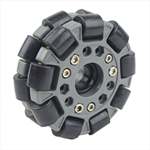
\includegraphics[width=.3\linewidth]{ANALYSIS/90degwheel.png}
					\caption{An omnidirectional wheel, with 90 degree rollers}
					\label{90 Degree Omni Directional Wheel}
				\end{figure}
				
				A robot chassis composing of three or four of these wheels as well as relevant motors should be adequate. A few of the different chassis found during the preliminary research will now be evaluated to find which would be the most suitable for the project.
				
					\subsubsection{3WD 48mm Omni-Directional Triangle Mobile Robot Chassis}
						\begin{figure}[h]
							\centering
							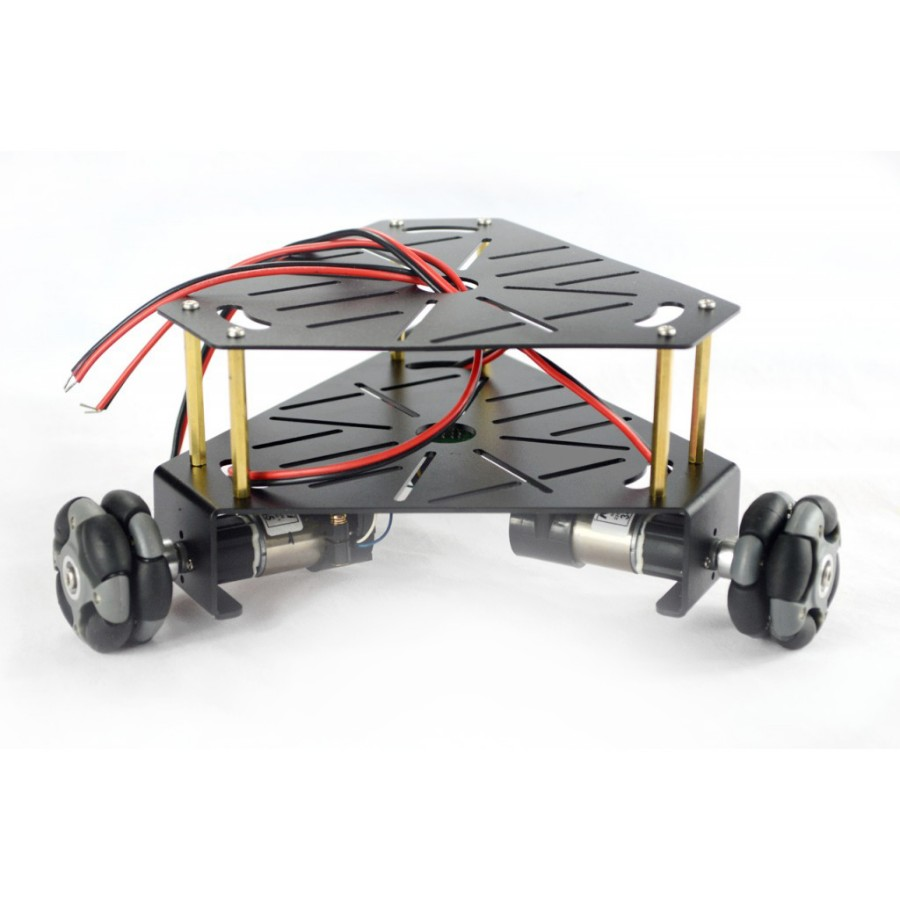
\includegraphics[width=.3\linewidth]{ANALYSIS/3wdomnidirectionalchassis.jpg}
							\caption{3WD Omni-Directional Robot Chassis}
							\label{3WD Omni-Directional Robot Chassis}
						\end{figure}
					
			
			\section{Observation}
			To achieve self navigation as well as mapping, the robot will need to take observations about its surrounding environment. In order to efficiently map the area and detect obstacles this will need to be performed in a 360 degree manner as well. This section aims to explore a few of the different methods that could be used for this, and ultimately to draw a conclusion on what method we will use.
			
				\subsection{Infrared}
				Infrared sensors work by measuring things via the reflection of infrared light. The sensor will send out some infrared light where it will be reflected off of an obstacle. A reciever will capture this reflected light and depending on factors such as how much light is recieved back and the triangulation of how the light was recieved the presence of an obstacle will be determined. There are a number of Infrared sensors available online for very cheap prices, websites like RobotShop and HobbyTronics list most of their sensors between £5 and £10. 360 sensors are incredible difficult to find, but their low price means purchasing a few would not be a problem.
				
				The range and degrees of space being measured will depend on the sensor's model, but there are a few things the different sensors have in common. First, infrared sensors have both a maximum and a minimum range. Not only does the maximum range need to be factored in as sensor will struggle to pinpoint the location of light that has been reflected at a large range, but the sensor will also struggle to 'see' very close obstacles. In addition, infrared sensors struggle in strong sunlight and seem best suited to primarily indoor tasks.
				
				
				\subsection{LIDAR}
				LIDAR (Light Detection And Ranging) is a technology that uses light sensors to measure distances between the sensor and the target object. It achieves this by sending out light pulses which bounce off of objects back at the sensor where they are collected.
				
				LIDAR has seen some popularity in mobile robotics and the decision to use LIDAR would give the project some interesting options. Some sensors boast very impressive statistics, with some ranges exceeding 10 metres whilst providing several thousand samples per second with 360 degree coverage \citep{slamtecA1M8}. Some of these sensors also feature SDKs (Source Development Kits), meaning the core sensor functionality will be accessible straight away allowing development to focus on the robot's logic rather than being bogged down in the belt and braces implementation of preliminary functionality. These features are expensive however, with some sensors being as high as £350.
				
				\subsection{Ultrasonic}
				Ultrasonic sensors function by sending out ultrasonic pulses and measuring the amount of time it takes for these pulses to bounce back. Because sonar is sound based rather than light based, it isn't negatively affected by aspects such as heat, colour or dust. Sensors can interfere with eachother however, sonar sensors sending and recieves pulses in close proximity to eachother can cause issues. A single robot is only being developed, but given that we may need multiple sensors to perform a full 360 degrees of observation this could cause some considerable complications. Sonar sensors can be found relatively cheap depending on the sensor, with sites like HobbyTronics and RoboShop featuring sensors as cheap as £6 ranging up to some that cost around £50.
				\medskip
				
				it would appear that LIDAR, whilst the most expensive option, is what will provde the project with the most functionality and ease of use. Here we will look at a few different LIDAR sensors that could be suitable for the project.
			
				
			
		
		\chapter{An Investigation Into SLAM}
			\section{Introduction}
			The development of a moving robot is only one half of the end product. As previously mentioned in the project's Terms of Reference the purpose of this project is also to develop a robot that is capable of self navigation and mapping. In order for this to be possible, the robot must be capable of using observations about its environment to build a map. Not only that, but it also must track its own location within this environment. This chapter aims to explore SLAM, a computing problem with research and implemented solutions that deal with exactly that.
		
			\section{What is SLAM?}
			SLAM stands for Simultaneous Localization and Mapping, and is something sometimes employed by mobile robots. Localization refers to the ability for the robot to be aware of its location within an environment, for example knowing where it is within a room. Mapping simply refers to building a map of the environment, such as the room the robot is in. SLAM is performing both of these tasks at the same time. Durrant-Whyte and Bailey\citep{durrant2006simultaneous}, both academics that have done extensive work in the field of mobile robotics, best sum it up as the ability for a mobile robot to be placed at an unknown location in an unknown environment and then both create a consistent map of the environment and be able to accurately determine its location within this map. Similar definitions can also be found in other articles \citep{choset2001topological, dissanayake2001solution}.
		
			\section{Uses of SLAM in Industry}
			There are a myriad of potential uses for SLAM, many of which can be seen within the wider industry. Commercially it has been used for products such as vacuum cleaners, Dyson for instance has a small automated vacuum cleaner called the 360 Eye which employs SLAM techniques to map the areas that it moves around and cleans. SLAM has seen many uses in archaeological contexts owing to its ability to perform exploration without risk to human life, one team \citep{clark2008archaeology} developed an underwater robot that used SLAM in order to map underwater cisterns that had been built thousands of years ago. The uses have not gone unnoticed by larger organisations. One of the research organisations within the USA's Department of Defense has held challenges (known as the DARPA Grand Challenge) offering cash prizes as incentives to create high value research. These challenges involve organisations submitting cars that are timed as they race around certain environments. NASA have also made use of it in the past, in 2007 they used an autonomous underwater robot \citep{carnegie2007sinkhole} employing SLAM to go to the bottom of the world's deepest sinkhole. The robot used sensors to generate a sonar map of the sinkhole's inner dimensions 318 meters below the surface.  The drone also tested technologies that could be used in other more extreme underwater environments such as the oceans under the crust of Europa, one of Jupiter's moons. This has led to increased interest being expressed in using SLAM for planetary rovers, which would allow for the mapping and navigation of different planet surfaces.
			\medskip
		
			\section{The SLAM Problem}
			Let's use some key notations to help break down the essentials of the SLAM problem. \newline
			\textbf{t} - Current time. \newline
			\textbf{x\textsubscript{t}} - Location and orientation of vehicle. \newline
			\textbf{u\textsubscript{t}} - Control vector, for example drive forward 1 metre.  \newline
			\textbf{m\textsubscript{t}} - True location of \textit{i}th landmark within the environment. \newline
			\textbf{z\textsubscript{t}} - Observation of \textit{i}th landmark taken at time \textit{t}.\newline
			
			From these notations we can derive some sets. \newline
			\textbf{x\textsubscript{0:t}} = $\lbrace$ \textbf{x\textsubscript{0:t-1}}, \textbf{x\textsubscript{t}} $\rbrace$ - History of all vehicle locations. \newline
			\textbf{u\textsubscript{0:t}} = $\lbrace$ \textbf{u\textsubscript{0:t-1}}, \textbf{u\textsubscript{t}} $\rbrace$ - History of odometrical information pertaining to teh robot's movement. \newline
			\textbf{m} = $\lbrace$ \textbf{m\textsubscript{1}}, \textbf{m\textsubscript{2}}, ..., \textbf{m\textsubscript{n}}$\rbrace$ - Set of all landmarks. \newline
			\textbf{z\textsubscript{0:t}} = $\lbrace$ \textbf{z\textsubscript{0:t-1}}, \textbf{z\textsubscript{t}} $\rbrace$ - Set of all landmark observations. \newline
			
			Ultimately we want to use the robot's control inputs and observations to receive a map of the environment and the robot's path.
			
			\begin{figure}[h]
				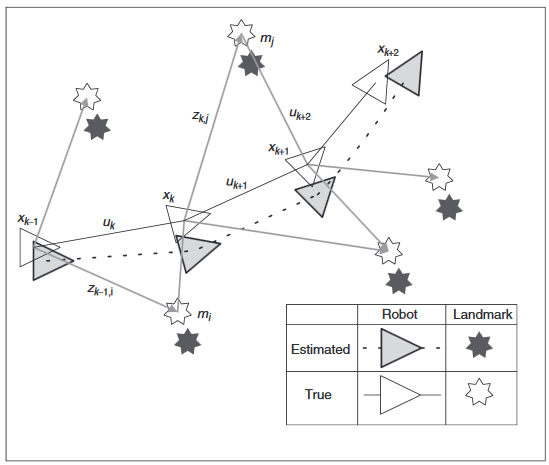
\includegraphics[scale=0.65]{ANALYSIS/slamdiagram.png}
				\caption{The SLAM problem illustrated \citep{durrant2006simultaneous}}
				\label{fig:slamillustration}
			\end{figure}
			
			SLAM is generally approached probabilistically. This means that the attempted solutions factor in uncertainties within the data. Therefore, solutions to the SLAM problem will not act with exact certainties. For example, rather than saying the robot is in an exact location we would treat it as a general location it is the most likely to be in. We want the probability distribution to be an estimation of current vehicle location and landmarks based on landmark observations and control inputs or odometrical data. 
			
			There are variations within the SLAM problem however. At a broader level, SLAM problems generally come in one of two flavours. These are full SLAM and online SLAM. 

				\subsection{Full SLAM}
				Full SLAM involves using landmark observations and data relevant to discerning the robot's current position in order to determine the robot's entire path. It can be written as such -
				
				p(\textbf{X\textsubscript{0:t}}, \textbf{m} $\mid$ \textbf{Z\textsubscript{0:t}}, \textbf{U\textsubscript{0:t}})
				
				\subsection{Online SLAM}
				Online SLAM differs slightly in that it seeks to determine the robot's current location rather than the robot's entire path. It can be written as such - 
				
				p(\textbf{x\textsubscript{0:t}}, \textbf{m} $\mid$ \textbf{Z\textsubscript{0:t}}, \textbf{U\textsubscript{0:t}})
				
				\subsection{SLAM Taxonomy}
				The possible differences in the SLAM problem don't end there. Depending on different factors there are also different sub approaches to the SLAM problem. Below are some common variants.
				
					\subsubsection{Volumetric versus Feature-Based}
					Volumetric SLAM samples the map as a resolution high enough to allow a photo realistic reconstruction of the environment \citep{thrun2008simultaneous}. The map gained from this is generally high dimensional, but as the area increases in size and scale the map becomes significantly more complex. Feature-based SLAM simply extracts key features from measurements, with the map being solely made up of these features. This might be used if it is decided that only key features are of interest or if large parts of the mapped space are empty, as volumetric SLAM in these cases would be storing voxels that hold no geometric data of significant value \citep{vespa2018efficient}. As you would expect, this is quicker and more efficient but discards a lot more data than volumetric. 
					
					\subsubsection{Topological versus Metric}
					Topological SLAM captures key places and their connectivity to other measured locations. Metric SLAM attempts to model the environment using geometrically accurate positioning. Metric SLAM would show the accurate positioning of various environmental features, topological would show them in relation to each other (e.g. place A is adjacent to place B) \citep{thrun2008simultaneous}. A good analogy would be a bus route map (topological) that displays the different stops versus showing the bus' actual route on a geographical map of the area (metric).
					
					\subsubsection{Known versus Unknown Correspondence}
					This entails relating the identity of sensed landmarks to other sensed landmarks. In known correspondence the identity of the landmarks is known, if a landmark is observed and then the robot moves and observed another landmark, the identity of the landmarks being known would let us to determine if this landmark observation is the one we saw before or a newly observed one. Unknown correspondence would simply mean that in this situation we wouldn't know.	
					
					\subsubsection{Static versus Dynamic}
					Static and Dynamic here refers to the environment. Static SLAM algorithms assume that no changes will take place in the environment whereas Dynamic SLAM methods allow for these changes to take place.
					
					\subsubsection{Small versus Large Uncertainty}
					The ability to represent uncertainty is another aspect. Some SLAM approaches will assume a very low uncertainty in the robot's location estimation. This might be when the robot is moving up and down a simple path, as it's much easier to guess where it's likely to be. Large amounts of uncertainty might occur however in more complex environments where locations can be reached from multiple different directions, or if the robot starts travelling in more complex paths that intersect with each other.
					
					
					\subsubsection{Activate versus Passive}
					Active SLAM involves the robot actively exploring its environment whilst it builds a map of it. Passive SLAM is when the SLAM algorithm is purely used for observation, with some other entity controls the robot's movement. 
					
					\subsubsection{Single-Robot versus Multirobot}
					Single-robot simply refers to SLAM happening only on a single platform. Multirobot SLAM (sometimes known as cooperative SLAM) involves multiple robots often communicating with each other to merge their maps into a larger collective model. 
				
					\medskip
					There are multiple different paradigms that can be used to solve the SLAM problem, and each of these paradigms has many different implementations. One technique that has seen usage for solving the SLAM problem in autonomous mobile robotics is the Canonical Scan Matcher, generally referred to as CSM. This is the solution that we will be looking to implement for the project.

			\section{A Look At A Potential Solution}
				\subsection{Introduction}
				As previously discussed there are a myriad of variations on the SLAM problem, and there are a few different paradigms used to implement solutions to it. During some preliminary research, one method of SLAMming came up that seemed like it would be suitable for the project called CSM.
				
				\subsection{CSM}
				CSM is an open-source C implementation of an ICP variant known as PlICP. It has seen usage for industrial prototypes of autonomous robotics, one of the most notable examples of this being Kuka, a German manufacturer of industrial robotics. It isn't quite a fully fledged SLAM solution, instead performing pairwise scan-matching on scan data that is fed into it. Before the PlICP algorithm it is based on can be explained, we must first look at the base ICP algorithm.
			
					\subsubsection{ICP}
					ICP stands for Iterative Closest Point, and it refers to an algorithm that attempts to minimize the difference between two clouds of points, something known as point matching or point set registration. In essence, it means getting one set of points aligned to another set of points. Besl and McKay present the algorithm as a statement \cite{besl1992method} in their paper, and ICP is shown in terms of C++ in the Mobile Robot Planning Toolkit \citep{mrpt2013icp}. 
					
					We first of all have a source map, and then we have a map that we wish to align to it which we will refer to as the reference map. We then go through each point in the source map and which point in the reference map is the closest to it. We then determine a transformation which would minimize the mean squared error (the average squared difference) between the two points before applying this transformation to the reference set and then going through this set of steps again. This is repeated until a the mean squared error falls below a certain threshold.
					
					\subsubsection{PlICP}
					Censi explains PlICP in a series of steps \citep{censi2008icp}. To start with, we take a reference scan, a second scan and a first guess for the translation needed to try and match the two maps. We then generate a polyline of the reference map by connecting sufficiently close enough dots (using a threshhold). Following this, a loop similar to the one in the base ICP algorithm begins.
					
					We first determine the coordinates of the second scan in the first scan's frame of reference using our initial translation guess. Then, for each point in the second scan, we determine the two closest points to it in the first scan. We trim any outliers within these matches, and use the sum of the squares of the distances from the points to the line containing the matches two points to find the error function. PlICP then uses an algorithm in order to minimize this error function which we now use as our translation guess. This new guess is used on the next iteration of the algorithm. This loop continues until either we have a convergence between the maps or a loop is detected as no further progress is being made.	
					
			\subsection{Suitability of CSM}
			Firstly we can see that CSM is a pure C implementation of the previously described algorithm. This is excellent for the project, not just for the benefits of C such as it being a relatively quick language but also because it should be directly usable with an embedded board which would be the ideal choice for controlling the robot. Had it been in any other language we might have needed to use some sort of shared library to get it to work which likely would have slowed things down and potentially made the robot less effective. 
			
			CSM is however not a product of a professional company dealing in these matters, its open source nature could put some doubts with regards to its usefulness or reliability. However, it was developed by Dr Andrea Censi, someone who is a Deputy Director for the Chair of Dynamic Systems and Control at ETH Zurich meaning it is far from an amateur project. As previously mentioned as well it has been adopted by the German robotics company Kuka, so clearly it has enough merit to be used at the industrial level. Ultimately it would appear CSM is an ideal choice for the robot's localization and mapping functionality.
					
			\section{An Investigation Into SLAM - Conclusions}	
			First and foremost we can safely establish that the SLAM problem is what we are addressing with regards to the implementation of the robot's ability to track its own location whilst mapping its environment. In addition to this we understand the fundamentals of the SLAM problem. This will massively benefit development, as being aware of having to store details internally such as wheel revelations gained via odometric sensors will allow us to cut down on time spent during development having to rewrite core pieces of functionality to make room for this. 

		%\chapter{Solutions}
		\chapter{Product Requirements}
		Look at the objectives from the TOR, outline what the robot and the software needs to do to achieve these objectives.
			
		
		
		\chapter{Review of Tools and Techniques}
			\section{Micro C}
			\section{MBED OS}
		
			\section{Scanning Behaviour}
			One aspect that needed to be considered was the drone's behaviour whilst scanning. The initial thought was that the drone would move around, scan and save the scan results all simultaneously. To investigate the viability of this tests were performed to see if this was possible with the constraints we had, the most notable constraints being how quickly the MBed board is able to write scan data compared to how quickly it would be receiving it from the LIDAR sensor. *!Have some numbers here describing the time it takes to write data retrieved from 1 seconds' worth of LIDAR scanning!*. Based on this it was decided it would be best if the LIDAR stopped and took readings for a small period of time, with these readings being stored in the RAM and then written to internal files afterward. 
			
			\section{Dead Reckoning}
			Odometry is the usage of data from motion sensors to estimate an object's position. One such implementation of this that will be looked at for the project is dead reckoning. Dead reckoning tracks the robot's position by using data from wheel encoders that count the number of wheel rotations performed during operation. From this, the internal tracked position of a robot can estimate its new position after periods of movement. Given that the chassis being used for the project has wheel encoders as part of the wheel motors, this approach would allow us to perform odometry without needing the use of additional kit. Dead reckoning is not without issues however. Most pressingly it does not account for wheel slippage. If the robot has a poor grip on the ground and the wheels slip, then the wheel rotation doesn't accurately correspond to the robot's location \citep{choset2001topological}. These issues would compound as well. As more and more slippage happens, the robot's internal position would become less and less accurate to where it actually is. 
				
	
	\part{Synthesis}
	\chapter{Introduction}
	Now that the relevant product fields are understood to a sufficient degree and the product's needs have been established we can begin to plan out how we will achieve the project's objectives. First we will established the methological approach that will structure the product's development. Then, for each of the core product requirements we will look at a high level design overview of how the requirement will be met, the actual implementation of this design, and testing to evaluate how well this requirement has been satisfied by this implementation.
	
	\chapter{Methological Approach}
	The project employed a prototyping methodology for development. First, we must perform an investigation into the system requirements, which was performed in the analysis with a list of specific core requirements being outlined in the conclusion. Following this the first prototype is built, which will resemble an incredibly basic scaled down version of how the final system should ideally look. This prototype is then thoroughly evaluated, with potential changes that would bring the prototype closer to the final system being figured out. Finally, these changes are then implemented and the prototype is evaluated once again. This is repeated until the product has reached its ultimate goals.
	
	%prototyping diagram?
	
	This methodology was employed partially due to the hardware nature of the product. Key features of the robot hinged on aspects like movement and observation being possible, so it was important to get a prototype that has this basic functionality up and working and quickly as possible. The prototyping approach allowed a pure focus on getting these functions working, and once they were the robot could be improved iteratively.
	
		\subsection{Initial Prototype}
		As previously stated, this methodology involves an initial prototype that all future prototypes will be an iteration of. The initial prototype of the project will involve the basic, primary construction of the robot. This will first involve the basic chassis assembly, followed by connecting relevant components to each other and then ensuring that they are all powered. Once this is done, we'll hopefully have an incredibly crude robot that won't be capable of much, but should hopefully serve as a solid foundation for future development toward the project goals.
		
		A similar approach will be followed for processing the map data. It won't be developed simultaneously at first as the robot needs to be capable of storing observational data from the LIDAR before the program can actually do anything, however it will start to be put together once the robot crosses this developmental threshhold.
	
	\chapter{Design}
	Before implementation of the specific project aims can be implemented, we first need the initial prototype that we can begin iteratively improving. Therefore, it's logical to design the initial robotic prototype first. What follows is an overview of how the initial robot prototype will be designed, followed by a breakdown of each of the individual project aims will be met.
	
		\section{Initial Prototype}
		Here will be the design for the base robot. The aim here is to achieve a solid foundation that all development can build on in order to meet the project objectives.
			\subsection{Hardware}
				\subsubsection{Chassis}
				First off will be the basic assembly of the three wheeled omnidirectional chassis. The chassis is comprised of two triangular metal plates, joined together by metal rods that are screwed into pre drilled holes that line up to eachother. The lower platform is where the motors and mounting points for the omnidirectional wheels are found, so once the plates have been connected the wheels will be pushed onto these mounting points and locked into place.
				% assembly diagram here?
				
				Now it's time for the microcontroller setup. The microcontroller used in this project is the FRDM-K64F, chosen for it's relatively low cost, small form factor and compatibility with the Micro C Operating System which is being employed for the robot's core program. To control the robot we'll also need a motor driver. The dfRobot Quad Motor Driver Shield is being employed for this project, it can be obtained from Amazon for around £13. It was chosen for this relatively low cost, the easily available documentation and the fact that it can easily plug into the FRDM-K64F, the microcontroller of choice for this project. The specifics behind how the shield will be used will be discussed during the movement design section, but in short it allows us to manipulate the energy being sent to the individual wheel motors which will afford us control over how they work and as such control over the robot's movement. Once these two components have been fitted together, the power and ground cables from each of the chassis motors will be plugged into the motor driver shield. Fig \ref{fig:shieldsetup} from the shield's documentation shows an example of this setup with four motors.
				
				\begin{figure}[h]
					\centering
					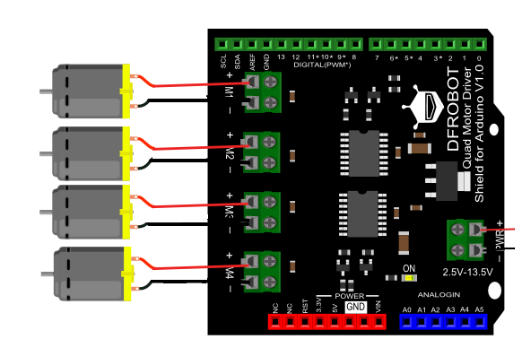
\includegraphics[width=.7\linewidth]{SYNTHESIS/shield_connection.png}
					\caption{Example shield setup}
					\label{fig:shieldsetup}
				\end{figure}
				
				The assembly shouldn't be overly complex, no soldering should be needed to connect components so it should be mostly a case of fitting things together.
				% explain LIDAR later.... :(
				
				\subsubsection{Power}
				The hardware components that will need powering are the three motors used to drive the omnidirectional wheels, the microcontroller, and the LIDAR sensor. The LIDAR sensor has two seperate pins that require power, one powering the motors that drives the LIDAR sensor and the other being the actual range finder itself. Table \ref{table:1} has a run down of these hardware components and the voltages that they use.
				
				\begin{table}[h!]
					\centering
					\begin{tabular}{|| l | l ||} 
						\hline
						Component & Voltage \\ [0.5ex] 
						\hline
						3x DC Coreless Motor  & 12V  \\ 
						FRDM-K64F  & 1.71 to 3.6V   \\
						RPLIDAR Scanner  & 5 to 5.5V  \\
						RPLIDAR Motor & 5 to 10V  \\ [1ex] 
						\hline
					\end{tabular}
					\caption{Components and respective voltages}
					\label{table:1}
				\end{table}
				
				To save on cost and complexity, it would be ideal to only use a single battery for the robot's power source. A single power source will be used for the robot, a battery holder containing 8 1.5V batteries will give us the 12V we need for the motors. Then, a step down voltage regular will be used to lower the voltage required for the other components. Fig \ref{fig:powersetup} has an overview of this.
				% !!!!!!!!!!!!!!!!!!!!!!!COME BACK TO THIS!!!!!!!!!!!!!!!!
			
			\subsection{Software}
			The software for the actual robot will be written in C++, compiled and deployed onto the microcontroller with the mbed SDK. At its foundation, it will be a Micro C OS with a series of configured tasks to perform various aspects of the robot's functionality. As you would expect, these tasks will come with their own memory tasks and will be designated with appropriate priorities. For the initial setup, we only need to make a skeleton OS to ensure we can properly compile and deploy code onto the microcontroller. Some relevant data structures and variables for task priorities and memory stacks, as well as a single task that prints hello world would be fine for this.
		
		\section{Designing for Requirements}
		Once this incredibly basic initial prototype is in place, we can begin to move toward truly fulfilling the project requirements. What follows is an overview of how each of the different project requirements will be met, with appropriate explanations toward the hardware and software employed.
		
			\subsection{Movement}
			The first of the three product aims outlined in the Analysis is that 'the robot must be capable of movement'.
				\subsubsection{Hardware}
				The previously mentioned dfRobot Quad Motor Driver Shield comes into play here. As shown in fig \ref{fig:shieldsetup}, the motors power and ground cables will connect to the appropriate pins on the shield. The motors can be manipulated once they receive power in this fashion. The shield is able to affect the electricity being sent to the motors by changing its polarity and by using pulse width modularity. By changing the pin to HIGH or LOW, we can affect the direction that the motor spins in (forward or backwards) and pulse width modulation allows us to affect the speed of the motor.
				
				\subsubsection{Software}
				In order to manipulate the motors we'll need some appropriate variables we can use to refer to the pins that the motor power and ground cables are connected to. %talk about pin lineup here and declaration
				
				% COME BACK TO THIS, TRIGONOMICAL NAVIGATION!

				
			\subsection{Observation}
				\subsubsection{Hardware}
				Only one range finder is being used to gather the observation data, the RPLIDAR A1M8 LIDAR sensor. The sensor is composed of a platform with a motor system that spins the range scanner as it takes readings, as well as some pins that can be used for communication. Fig \ref{fig:rplidarconfig} illustrates these components.
				
				\begin{figure}[h]
					\centering
					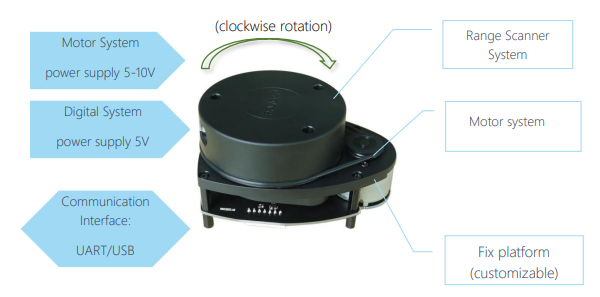
\includegraphics[width=.9\linewidth]{SYNTHESIS/rplidar_configuration.png}
					\caption{Example shield setup}
					\label{fig:rplidarconfig}
				\end{figure}
				
				\subsubsection{Software}
			\subsection{Processing Observational Data}
	
	\section{Designing for Requirements}
	%mention encoders?
		\subsection{Movement}
			
			\subsubsection{Hardware}
			\subsubsection{Software}		
			
		For this, the three wheeled omni directional chassis will be employed. This chassis was chosen due to the reduced cost compared to most other available chassis, and the omnidirectional wheels were ideal as the holonomic properties of the robot will allow it to move in any direction from any position without the need to first change its heading. To control the motors that will drive the wheels, the FRDM K64F MBED microcontroller will be used. The board is small, relatively cheap and will support the Micro-C Operating System that is going to be used as a structure for the robot's program. The motor driver
			
		From this, the robot will achieve an ability to move around an environment using basic navigation and the first of our three objectives will be met.
			
		\subsection{Observation}
		The second of the three product aims is that 'the robot must be capable of observation'.
			
		The RPLIDAR A1M8 360 Degree Laser Scanner will be used for the range finding aspect of this. Chosen for its high scan frequency and readily available SDK, it will be connected to the appropriate microcontroller pins so that it can recieve power and exchange information over a serial connection.
			
		This will allow the microcontroller access to range finding data and make it capable of utilizing the LIDAR sensor to observe the environment. A successful implementation here will achieve the second of our three product objectives.
			
		\subsection{Processing Observational Data}
		The last of the three product objectives is that 'the robot must be capable of processing observational data'.
		
		The plan for this is to use the CSM software described in the Analysis to process the robot's observational data. Once the robot has taken its observations, they will be saved onto an SD card that has been plugged into the FRDM K64F microcontroller. These observations will then be plugged into a computer where a created program will (once the user has directed it to) load this data and feed it into the CSM software. Once CSM has output an appropriate map, the program will display this to the user.
		
		Following a successful implementation of the above procedure, we will be capable of taking observational data and processing it into a viewable map. This will satisfy the last of the three project requirements.
	
	\medskip
	Now that we have a high level understanding of how each of the project objectives will be met, there will be a more thorough planning of how each of the hardware and software components will be implemented.
	
	% QUESTION - Should I discuss the cost of things here?
	\section{Hardware}
	This section aims to outline the hardware components selected for the project and to describe in a more detailed manner how the robot itself will be constructed.
	
		\subsection{Chassis}
			\subsubsection{Structure}
			The chassis is made up of an upper and a lower triangular platform, connected by small metal rods that screw into pre-drilled holes on the platforms. The lower platform features three 12 volt motors as well as mounting points for the omnidirectional wheels, which should lock into place once they are pressed onto it. %!! PUT ASSEMBLY DIAGRAM HERE?
			The space between the two platforms is where the robot's microcontroller and power supply will be housed, and the bulk of any wiring that needs to be done should ideally be here as well. On top of the upper chassis platform will be the LIDAR sensor used for range finding. It's important that the top platform remain relatively clean, as components or wiring being too close to the LIDAR may block the light it sends out and cause issues with the range finding process.
			
			The assembly shouldn't be overly complex, no soldering should be needed to connect components so it should be mostly a case of fitting things together.
			
			
			
		\subsection{Microcontroller}
			\subsubsection{FRDM-K64F}
			The FRDM-K64F will be employed to be the 'brain' of the robot. It's small, relatively cheap and compatible with the Micro C operating system which will run the tasks needed to be used for the robot's operation. As well, the freely available mbed SDK used for developing on these boards will make changing and redeploying code onto microcontroller quick and easy, which will help minimize time spent programming the next prototype iteration.
			
			\subsubsection{dfRobot Quad DC Motor Driver Shield}
			To manipulate the robot the way we want, we cannot simply supply all the wheels with full power all the time. This will make them constantly spin at the maximum rate. Omnidirectional navigation relies on having different wheels spin in different directions, often at different speeds. To achieve this, the motor driver shield will sit on top of our microcontroller. It features pins for each of the chassis motor's power and ground cables, and once plugged in we can run code on the microcontroller to change whether these pins are HIGH and LOW as well as the pulse width modulation of these pins. It was chosen for its ease of use and available documentation, as well as its immediate compatibility with the FRDM-K64F, installation will be as easy as plugged it into the board's GPIO pins. This will allow us to change both the direction and the speed of each of the individual wheels, which will help us achieve our omnidirectional navigation.
		
		\subsection{Sensor}
		The RPLIDAR A1M8 sensor will sit on top of the chassis and will be connected to the microcontroller. The microcontroller will provide the LIDAR with power, and a serial connection between the two components will allow the microcontroller to send and recieve information from the sensor. As mentioned in the power section, the LIDAR features two different pins that require power. These are the LIDAR motor and the LIDAR core, and they will recieve power that has been stepped down from the 12V battery pack that is being used.
	
	\section{Software}
		\subsection{Robot}
		The software for the actual robot will be written in C++, compiled and deployed onto the microcontroller with the mbed SDK. At its foundation, it will be a Micro C OS with a series of configured tasks to perform various aspects of the robot's functionality. As you would expect, these tasks will come with their own memory tasks and will be designated with appropriate priorities.
		
			\subsubsection{Sensor}
			In order to interface with the RPLIDAR A1M8, SLAMTEC's own SDK will be used. The SDK comes in the form of header files which appropriately implement the functionality needed to send requests and recieve information from the LIDAR sensor. Table \ref{table:3} has a manifest of the SDK and the functionality that it provides.
			
			\begin{table}[h!]
				\centering
				\begin{tabular}{|| l | l ||} 
					\hline
					File & Purpose \\ [0.5ex] 
					\hline
					rplidar.h  & Parent file for subsequent header files  \\ 
					rplidar\textunderscore driver.h  & Provides RPLidarDriver class for  interfacing with sensor   \\
					rplidar\textunderscore  protocol.h  & Defines structs and constants for the LIDAR protocol  \\
					rplidar\textunderscore  cmd.h & Defines request/answer structs for LIDAR protocol  \\ 
					rptypes.h & Platform independent structs and constants  \\ [1ex] 
					\hline
				\end{tabular}
				\caption{RPLIDAR SDK files}
				\label{table:3}
			\end{table}
		
		
		\subsection{Map Building}
	
		\subsubsection{FRDM-K64F}
		The FRDM-K64F will be employed to be the 'brain' of the robot. It's small, relatively cheap and compatible with the Micro C operating system which will run the tasks needed to be used for the robot's operation. As well, the freely available mbed SDK used for developing on these boards will make changing and redeploying code onto microcontroller quick and easy, which will help minimize time spent programming the next prototype iteration.
	
		\subsection{Sensor}
		The RPLIDAR A1M8 sensor will sit on top of the chassis and will send data to the microcontroller over a serial connection. Once this connection has been established, the microcontroller will be able to send request to the LIDAR. An overview of the possible requests that can be sent to the LIDAR can be seen in table \ref{table:2}.
		
		\begin{table}[h!]
			\centering
			\begin{tabular}{|| l | l ||} 
				\hline
				Function & Purpose  \\ [0.5ex] 
				\hline
				Scan & Begin scanning  \\ 
				Stop & Stop scanning  \\
				Reset & Reboot RPLIDAR core  \\
				Force Scan & Begin scanning without checking rotation speed  \\
				Get Info & Output device info (e.g. serial number)  \\
				Get Health & Output device health info  \\
				Get Samplerate & Output single sampling time  \\
				Get Lidar Conf & Get LIDAR configuration  \\ [1ex] 
				\hline
			\end{tabular}
			\caption{RPLIDAR SDK overview}
			\label{table:2}
		\end{table}
		

		
	\chapter{Implementation}
	\chapter{Testing}
	\part{Evaluation}
	\chapter{Introduction}
	The Evaluation chapter aims to determine the strengths and weaknesses of the project. The choice of equipment and techniques will be evaluated, taking into account their original reasons for being employed and how useful they were during the project's development. In addition the strengths and weaknesses of the project's approach will be evaluated. Situations where the project's approach allowed for progress to be made or obstacles overcome will be described, as well as incidents where something different may have yielded more success. Finally the product itself will be evaluated. The original project requirements outlined in the analysis will be touched on again, and then the matter of whether or not they have been satisfied will be discussed. Attention will be given to aspects such as the original reasoning behind the objectives, the preliminary research (or possibly lack thereof) that contributes to the objectives success/failure as well as any strengths or faults during the project's synthesis. Finally, some conclusions on the project will be reached followed by recommendations for further work in the same vein. 
	
	\chapter{Process Evaluation}
	%fitness for purpose and build quality sections from tor
	
	%talk about obvious issues with attempting to implement the SDK - get the actual linux error message(s)?
	%gives examples of previously attempted solutions and code snippets, e.g
	%i tried implementing manual getc and putc *actual code*
	%i tried using a byte lookup table on this *actual code*
	%i tried implementing a non-blocking interrupt handler attached to the rx channel *actual code*
	The way in which the project was approached had some strengths. The preliminary research into the relevant project fields prior to development helped in understanding what it was that precisely needed to be done to achieve the project goals.
	
	One of the biggest issues in the project was a grossly inefficient usage of time. The obstacle of establishing communication between the LIDAR sensor and the microcontroller came up right near the start of the project, but it was a great length of time before any actual success in having the two devices interface with eachother was realized. 
	
	\chapter{Product Evaluation}
	
	
	\chapter{Conclusions and Recommendations}
	\bibliographystyle{plainnat}
	\bibliography{papers}
	\part{Appendices}
	\begin{appendices}
	\chapter{Terms of Reference}
	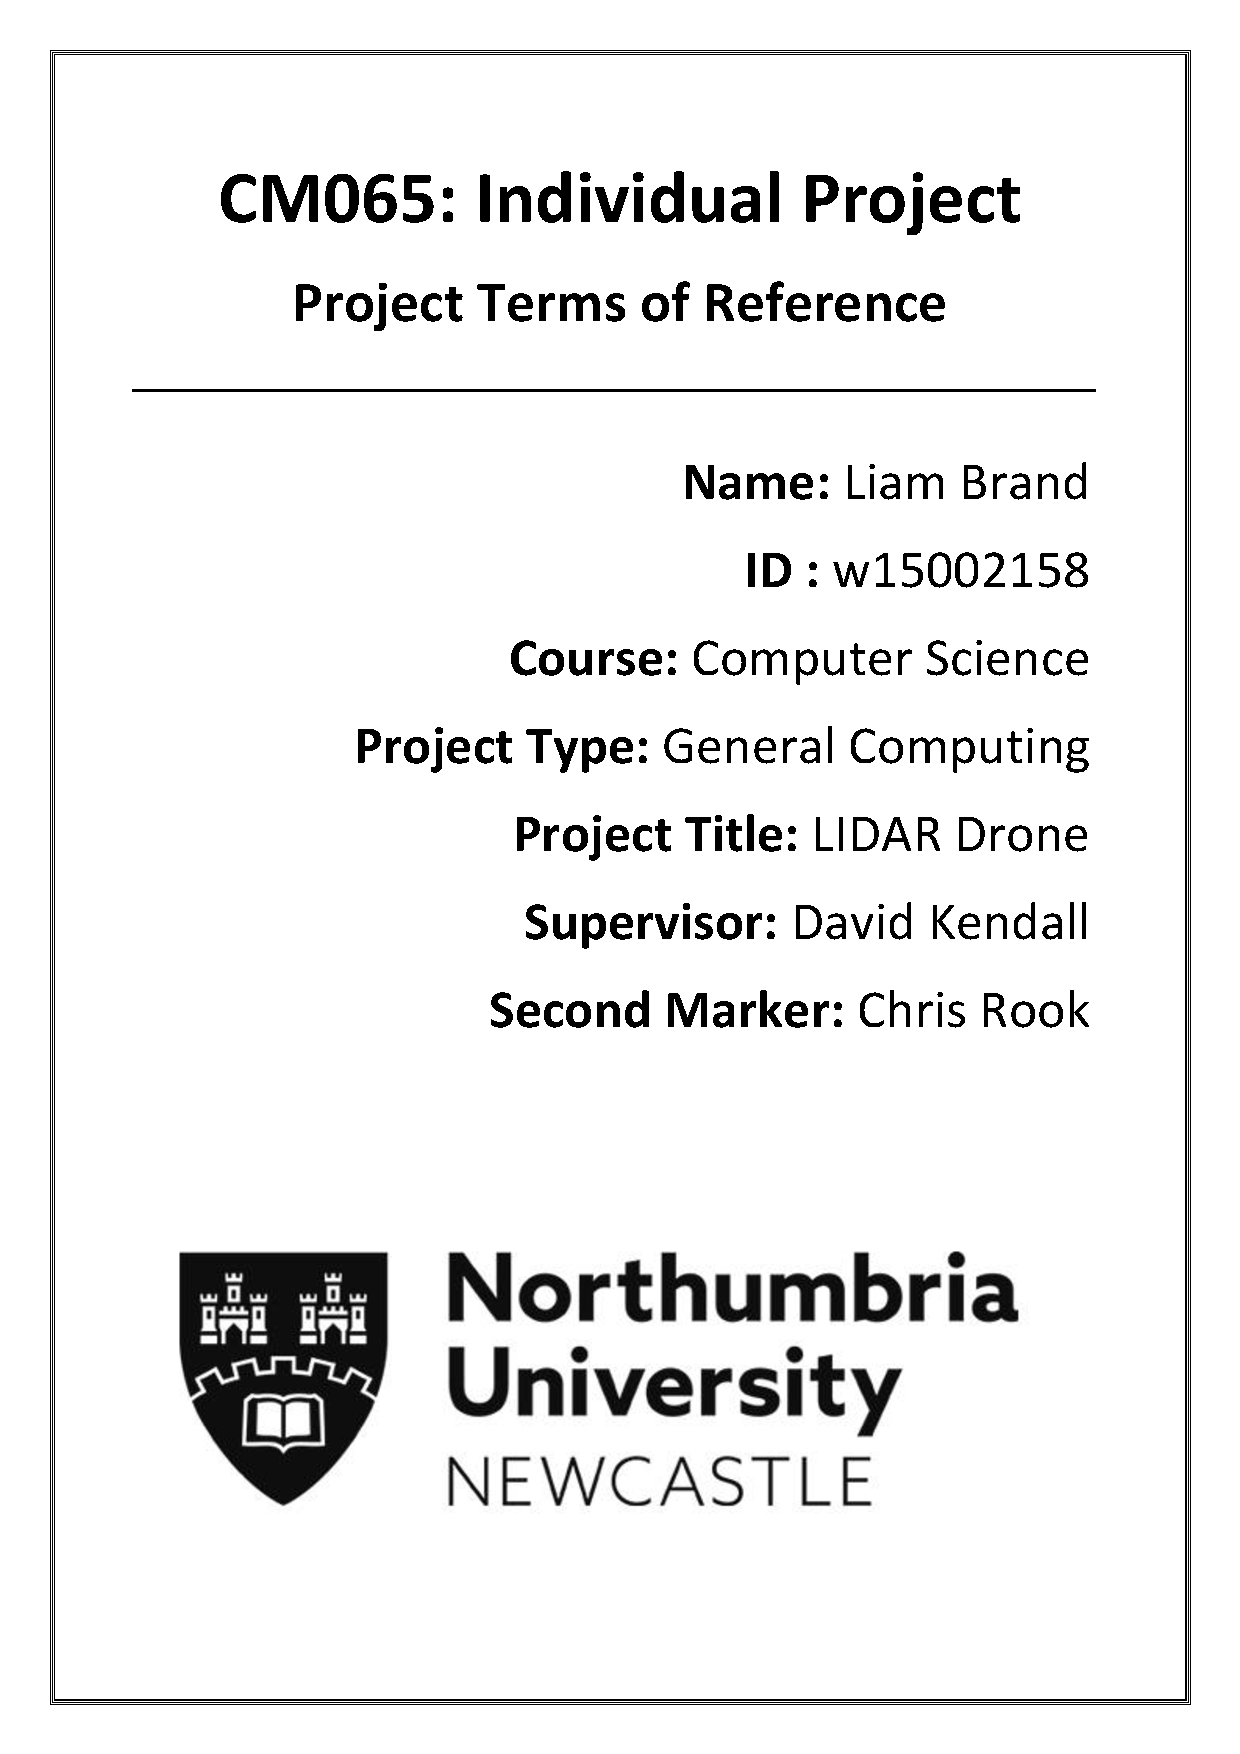
\includepdf[pages=-]{APPENDICES/TOR.pdf}
	\chapter{Program Code}
		\subsection{Robot Software}
			\subsubsection{main.cpp}
			Code repository can be found at: \url{https://github.com/liambrand/lidar-robot}
			\lstinputlisting[caption=main.cpp]{APPENDICES/main.cpp}
		\subsection{GUI}
			\subsubsection{mapgui.py}
			Code repository can be found at: \url{https://github.com/liambrand/robot-map-gui}
			\lstinputlisting[caption=mapgui.py, language=python, showstringspaces=false]{APPENDICES/mapgui.py}
	\chapter{Testing}
	\begin{landscape}
	\label{testingappendices}
		\label{testing:testlogs}
					\begin{table}[h!]
						\centering
						\begin{tabular}{| l | l | l |} 
							\hline
							Printed Direction & Direction Moved In & Test Result  \\ [0.5ex] 
							\hline
							Right & Right & Pass   \\
							Left & Left & Pass   \\ 
							Forward & Forward & Pass   \\ 
							Left & Left & Pass   \\ 
							Right & Right & Pass   \\ 
							Forward & Forward & Pass   \\ 
							Right & Right & Pass   \\ 
							Left & Left & Pass   \\ 
							Backward & Backward & Pass   \\ 
							Forward & Forward & Pass   \\ 
							Backward & Backward & Pass   \\ 
							Left & Left & Pass   \\ 
							Right & Right & Pass   \\ 
							Right & Right & Pass  \\ 
							Backward & Backward & Pass   \\ 
							Forward & Forward & Pass   \\ 
							Forward & Forward & Pass  \\ 
							Backward & Backward & Pass  \\ 
							Right & Right & Pass   \\ 
							Forward & Forward & Pass   \\ 
							Backward & Backward & Pass   \\ [1ex] 
							\hline
						\end{tabular}	
					\caption{Movement Integration Tests}
					\label{table:movementtestsbasic}	
					\end{table}
				
					\begin{table}[h!]
						\centering
						\begin{tabular}{| p{2.5cm} | p{5cm} | p{4cm} | p{3cm} | p{1.5cm} |} 
							\hline
							Test & Test Purpose & Expected Result & Actual Result & Pass/Fail \\ [0.5ex] 
							\hline
							Begin sensor & Determine microcontroller's ability to start LIDAR sensor & Sensor starts spinning & As expected & Pass  \\
							
							Output reading & Determine ability to retrieve data from the LIDAR sensor & Terminal prints scan data & As expected & Pass \\
							 
							Stop sensor & Determine microcontroller's ability to stop LIDAR sensor & Sensor stops spinning & As expected & Pass   \\ [1ex] 
							\hline
						\end{tabular}	
					\caption{LIDAR Integration Tests}	
					\label{table:lidartestbasic}
					\end{table}
				
					\begin{table}[h!]
						\centering
						\begin{tabular}{| p{2.5cm} | p{5cm} | p{4cm} | p{3cm} | p{1.5cm} |} 
							\hline
							Test & Test Purpose & Expected Result & Actual Result & Pass/Fail \\ [0.5ex] 
							\hline
							File Creation & Ensure the robot can create files & File present on Micro SD-Card & As expected & Pass  \\
							
							Basic File Writing & Ensure created file contains data & File shouldn't be empty & As expected & Pass \\
							
							Accurate Data & Ensure written data is what the LIDAR has produced & File's data should match what has been output on the terminal & As expected & Pass \\ 
							
							Intense File Writing & See if the system can cope with writing many thousands of readings & File should contain more data, system task should still finish as normal & As expected & Pass \\
							[1ex] 
							\hline
						\end{tabular}
					\caption{File Writing Integration Tests}
					\label{table:filewritingtests}		
					\end{table}
				
					\begin{table}[h!]
						\centering
						\begin{tabular}{| p{2.5cm} | p{5cm} | p{4cm} | p{3cm} | p{1.5cm} |} 
							\hline
							Test & Test Purpose & Expected Result & Actual Result & Pass/Fail \\ [0.5ex] 
							\hline
							GUI Starts & Ensure the GUI starts properly & GUI will start up after being called from the command line & As expected & Pass  \\
							
							File Readings & Ensure the GUI can process the given file & GUI shouldn't encounter errors processing values from the file & As expected & Pass \\
							
							Basic Map Generated & Ensure a basic map can be generated  & GUI should display a map of the environment the robot mapped & Map was not accurate & Fail \\ 
							
							CSM Map Generated & Ensure the GUI can use CSM to generate a map  & GUI should output a map incorporating multiple scans & No such functionality implemented & Fail \\ [1ex] 
							\hline
						\end{tabular}
						\caption{Mapping Integration Tests}
						\label{table:mappingtests}		
					\end{table}
				
					\centering
					\begin{longtable}{| p{2.5cm} | p{5cm} | p{4cm} | p{4cm} | p{1.5cm} | p{2cm} |} 
						\caption{System Tests}
						\label{systemintergrationtestingtable} \\
						\hline
						Test & Test Purpose & Expected Result & Actual Result & Pass/Fail & Comments \\ [0.5ex] 
						\hline
						Drive Forward & The robot should move forwards during its operation & As expected & The robot moved forwards when it was switched on & Pass & Hardcoded movement  \\
	
						Drive Right & The robot should move right during its operation & The robot is able to move right & The robot couldn't move right & Fail &   \\
							
						Drive Left & The robot should move left during its operation & The robot is able to move left & The robot couldn't move left & Fail &   \\
						
						Obstacle Avoidance & The robot should navigate around obstacles during operation & The robot is able to avoid obstacles & The robot didn't detect obstacles & Fail &   \\
							
						Motor Obstructions & During the previous drive tests, there should be no obstructions to the motors from the robot's other components & As expected & The robot's motors didnt get blocked & Pass &   \\
						
						Power Failured & During the previous drive tests, there should be no power issues & Robot will complete operation without issue & Microcontroller battery's GND cable slips out & Fail &   \\
							
						Scanning & The robot should stop to scan & The robot stops and scans its environment & As predicteda & Pass &   \\ 
							
						Write Scan Data & Ensure the robot can write scanned data to the Micro SD-Card & The Micro SD-Card will contain a file with scan data & As expected & Pass & Plugged in and viewed with USB adapter  \\
							 
						Writing Duration & Ensure the robot writes data to the Micro-SD Card in a reasonable time  & Writing should be done in under ten seconds & As expected & Pass &   \\ 
							
						Generate Map & Using the robot's scan data, the GUI should produce a basic map & Map will be produced resembling the robot's environment & Map was produced but didn't resemble the environment & Fail &  \\ 
							
						Generate Map Without File & Make the GUI attempt to generate a map without an available file & GUI will catch and handle a runtime exception & As expected & Pass &  \\ 
							
						Map Multiple Areas & Mapping should work on multiple different environments & Each map will be accurate to the environment the robot was in & Maps didn't resemble the environment & Fail &  \\ 
							
						Repeated Mapping & Repeated maps of the same area should look similar & Map will be produced resembling the robot's environment & Maps didn't resemble the environment & Fail &  \\ 
							
						SLAM & The system should be capable of producing a dynamic map using multiple scans from different locations & The GUI creates a map from the robot's scan data & No such functionality & Fail &  \\ [1ex] 
							\hline
					\end{longtable}
			\end{landscape}			

		\section{Test Code}
		\label{testing:testcode}
			\subsection{Basic Movement Testing}
			\label{testcode:movementbasic}
			\begin{lstlisting}
while (true) {
	// Random number between 0 and 3
	int r = rand() % 4;
					
	if(r == 0) {
		pc.printf("Forward");
		goForward();
	}
					
	if(r == 1) {
		pc.printf("Right");
		goRight();
	}
					
	if(r == 2) {
		pc.printf("Back");
		goBackward();
	}
					
	if(r == 3) {
		pc.printf("Left");
		goLeft();
	}

	OSTimeDlyHMSM(0,0,3,0);
}
			\end{lstlisting}
			
			\subsection{LIDAR Testing}
			\label{testcode:observation1}
			\begin{lstlisting}
static void appTaskLidarTest(void *pdata) {
	dtr = 0;
	rplidar.begin(lidar_device);
	rplidar.startScan();
	struct RPLidarMeasurement measurement;
				
	while (true) {
		dtr = 1;
		rplidar.waitPoint();
		measurement = rplidar.getCurrentPoint();
		pc.printf("Distance: %f Angle:%f\n", measurement.angle, measurement.distance);
		dtr = 0;
		OSTimeDlyHMSM(0,0,1,0);
	}
}
			\end{lstlisting}
			
			\subsection{SDFileSystem Testing}
			\label{testcode:filewriting2}
			\begin{lstlisting}
dtr = 1;
rplidar.begin(lidar_device);
rplidar.startScan();
struct RPLidarMeasurement measurement;
				
static void writeTest() {
	struct RPLidarMeasurement measurement;

	// Create the readings file on the Micro SD-Card
	FILE *fp = fopen("/sd/readings.txt", "w");
					
	// Log if the file cannot be made
	if (fp == NULL) {
		pc.printf("Unable to access/create file \n");
	}

	for(int i = 0; i < 10; i++) {
		lidar.waitPoint();
		measurement = lidar.getCurrentPoint();
		pc.printf("Angle:%f Distance:%f\n", measurement.angle, measurement.distance);
		fprintf(fp, "%f %f\r\n", measurement.angle, measurement.distance);
	}
					
	// Close file
	fclose(fp);
}
			\end{lstlisting}
	
	\chapter{Hardware Documents}
	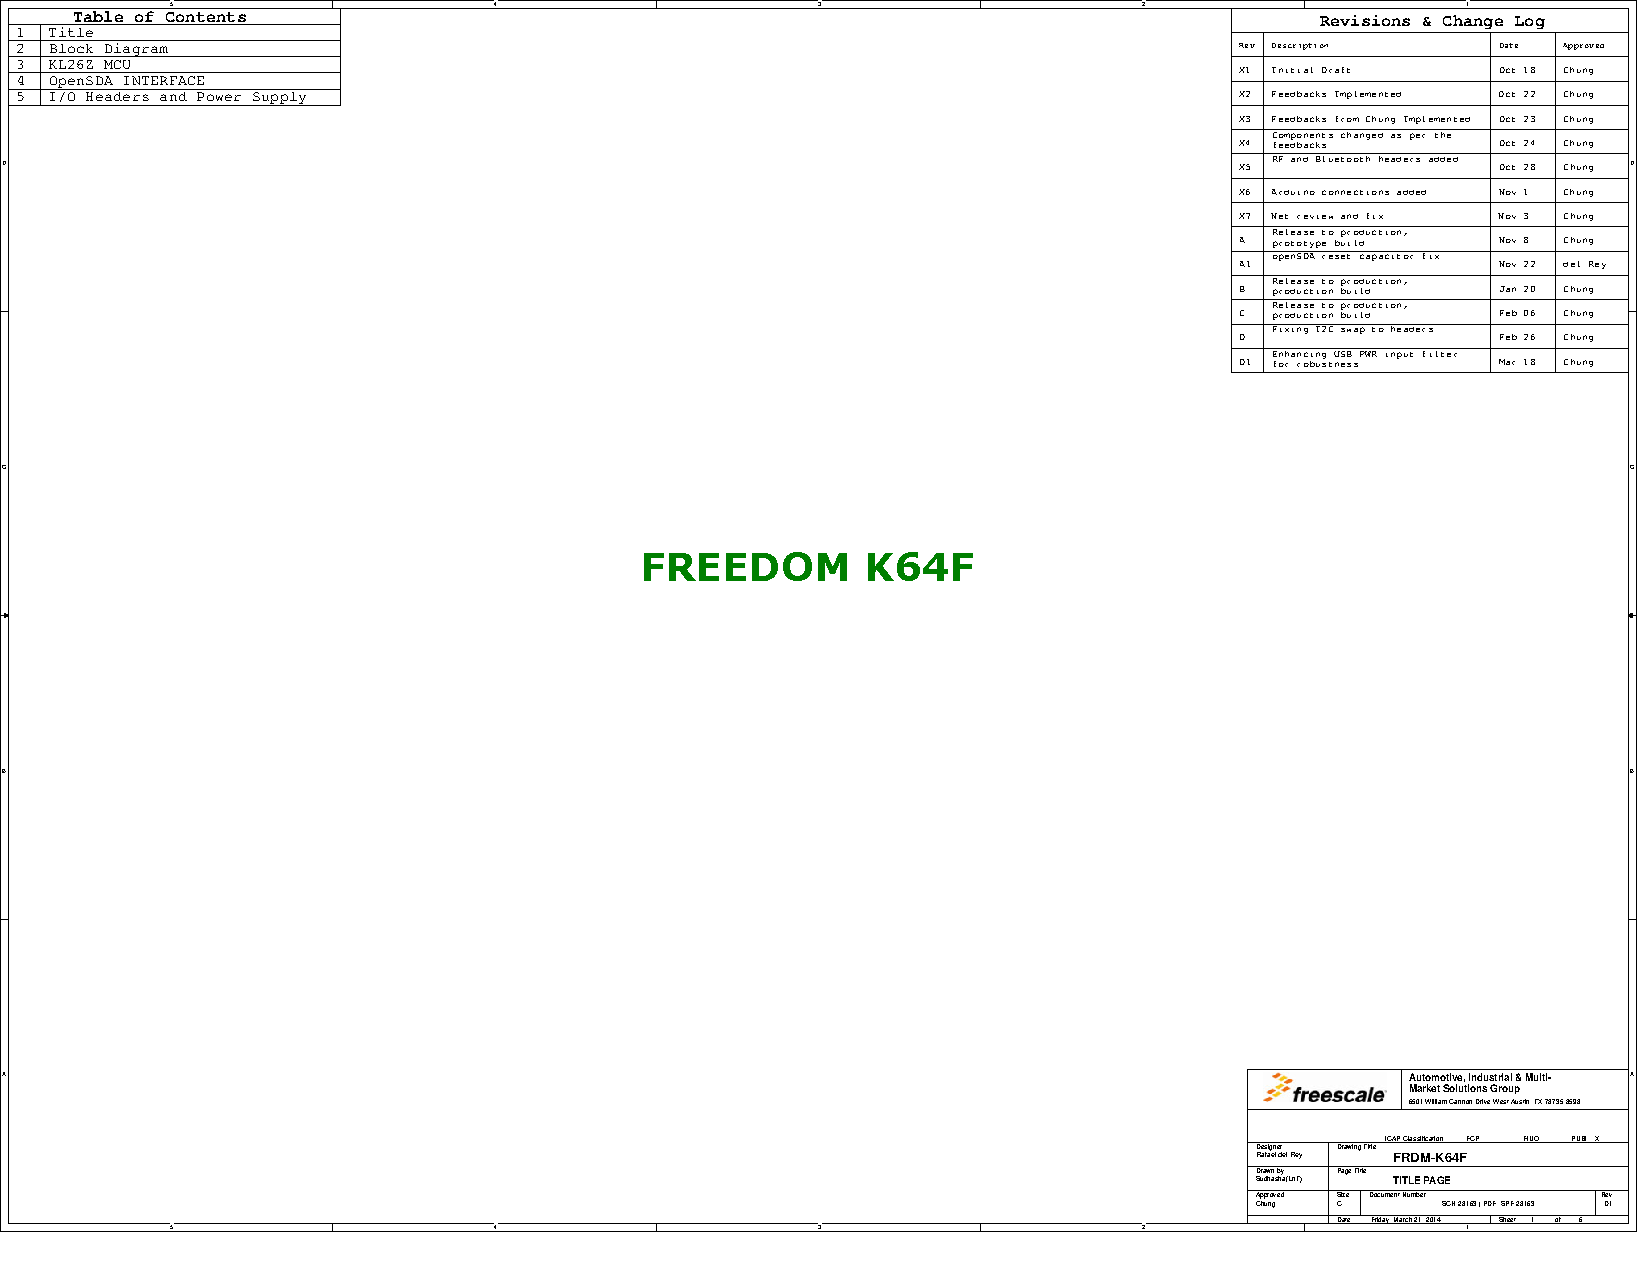
\includepdf[pages=-]{APPENDICES/k64fcircuitdiagram.pdf}
	\chapter{Ethics Form}
	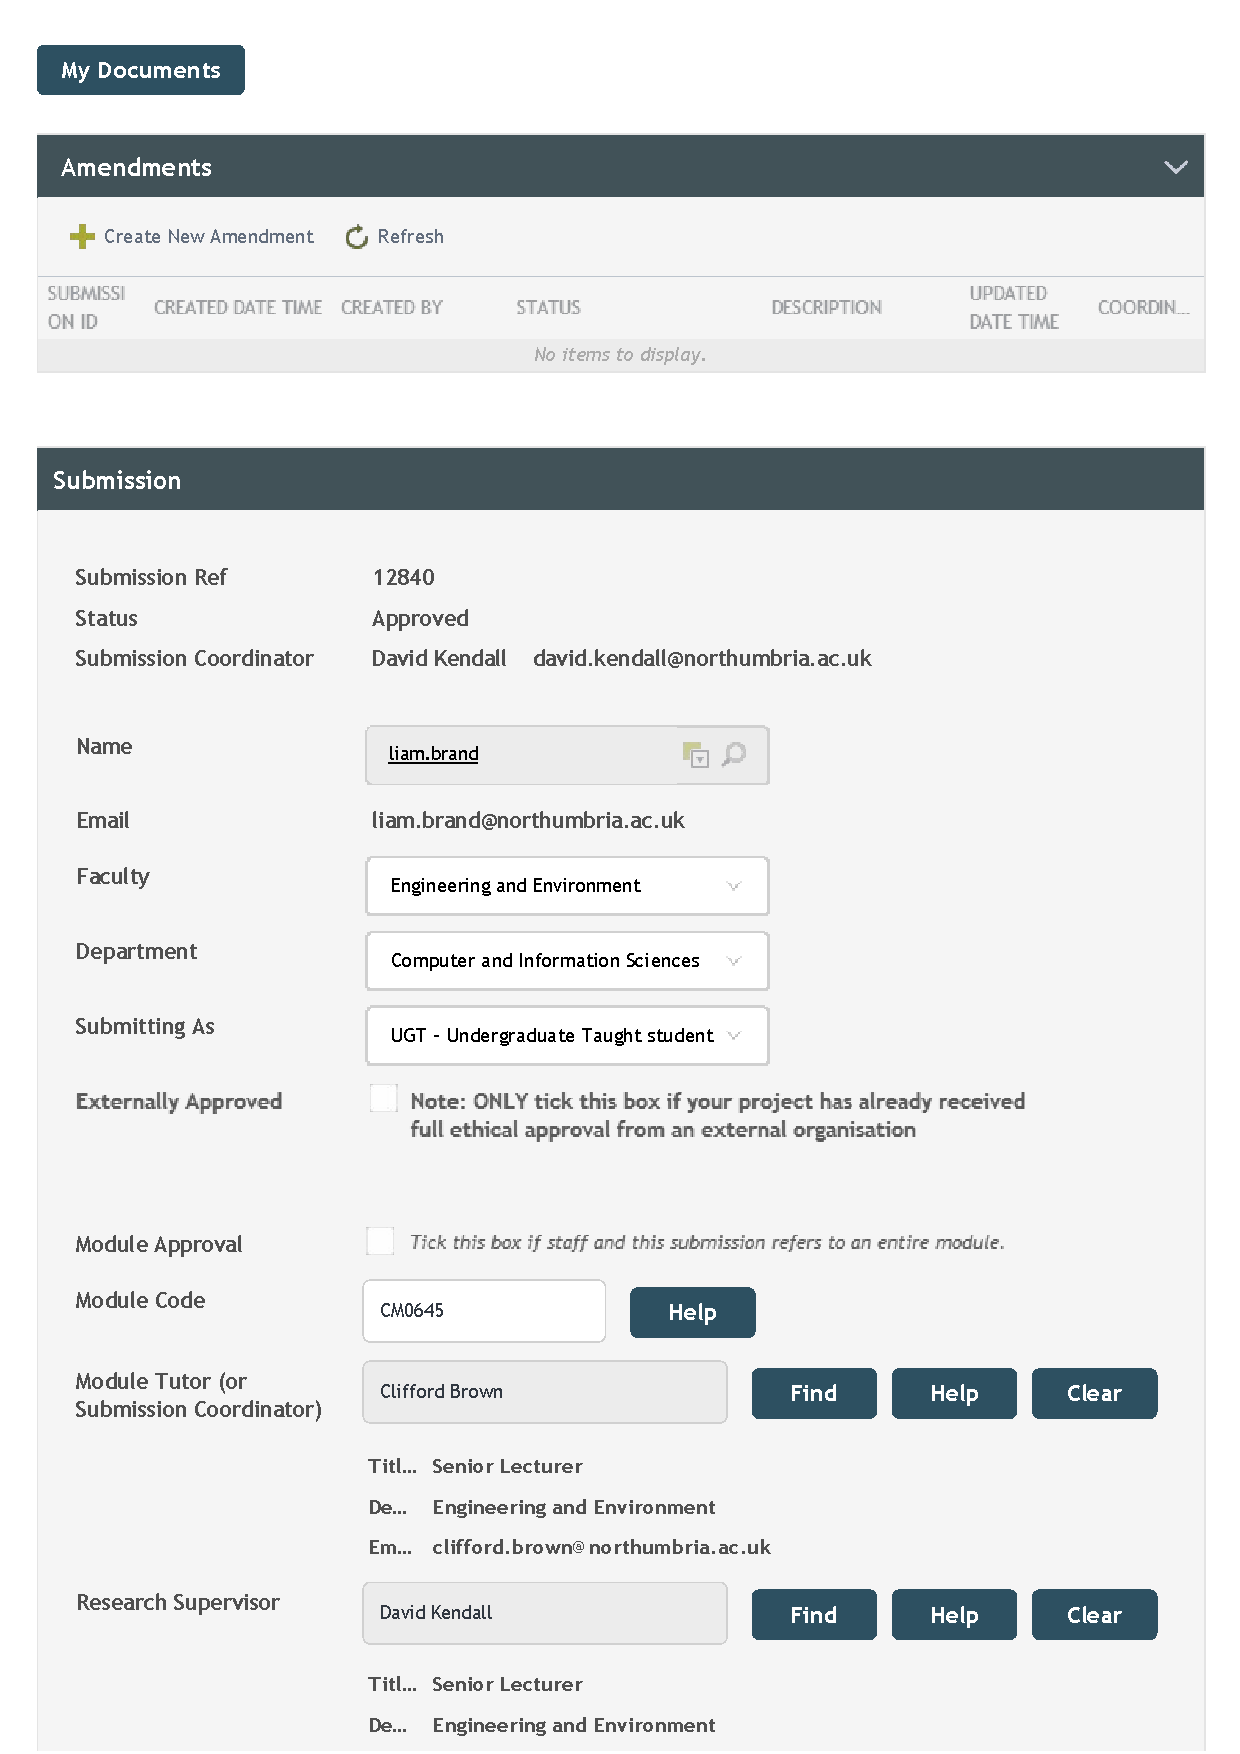
\includepdf[pages=-]{APPENDICES/ethicsonlineform.pdf}
	\end{appendices}
			

	%\part{Appendices}
	\begin{appendices}
	\chapter{Terms of Reference}
	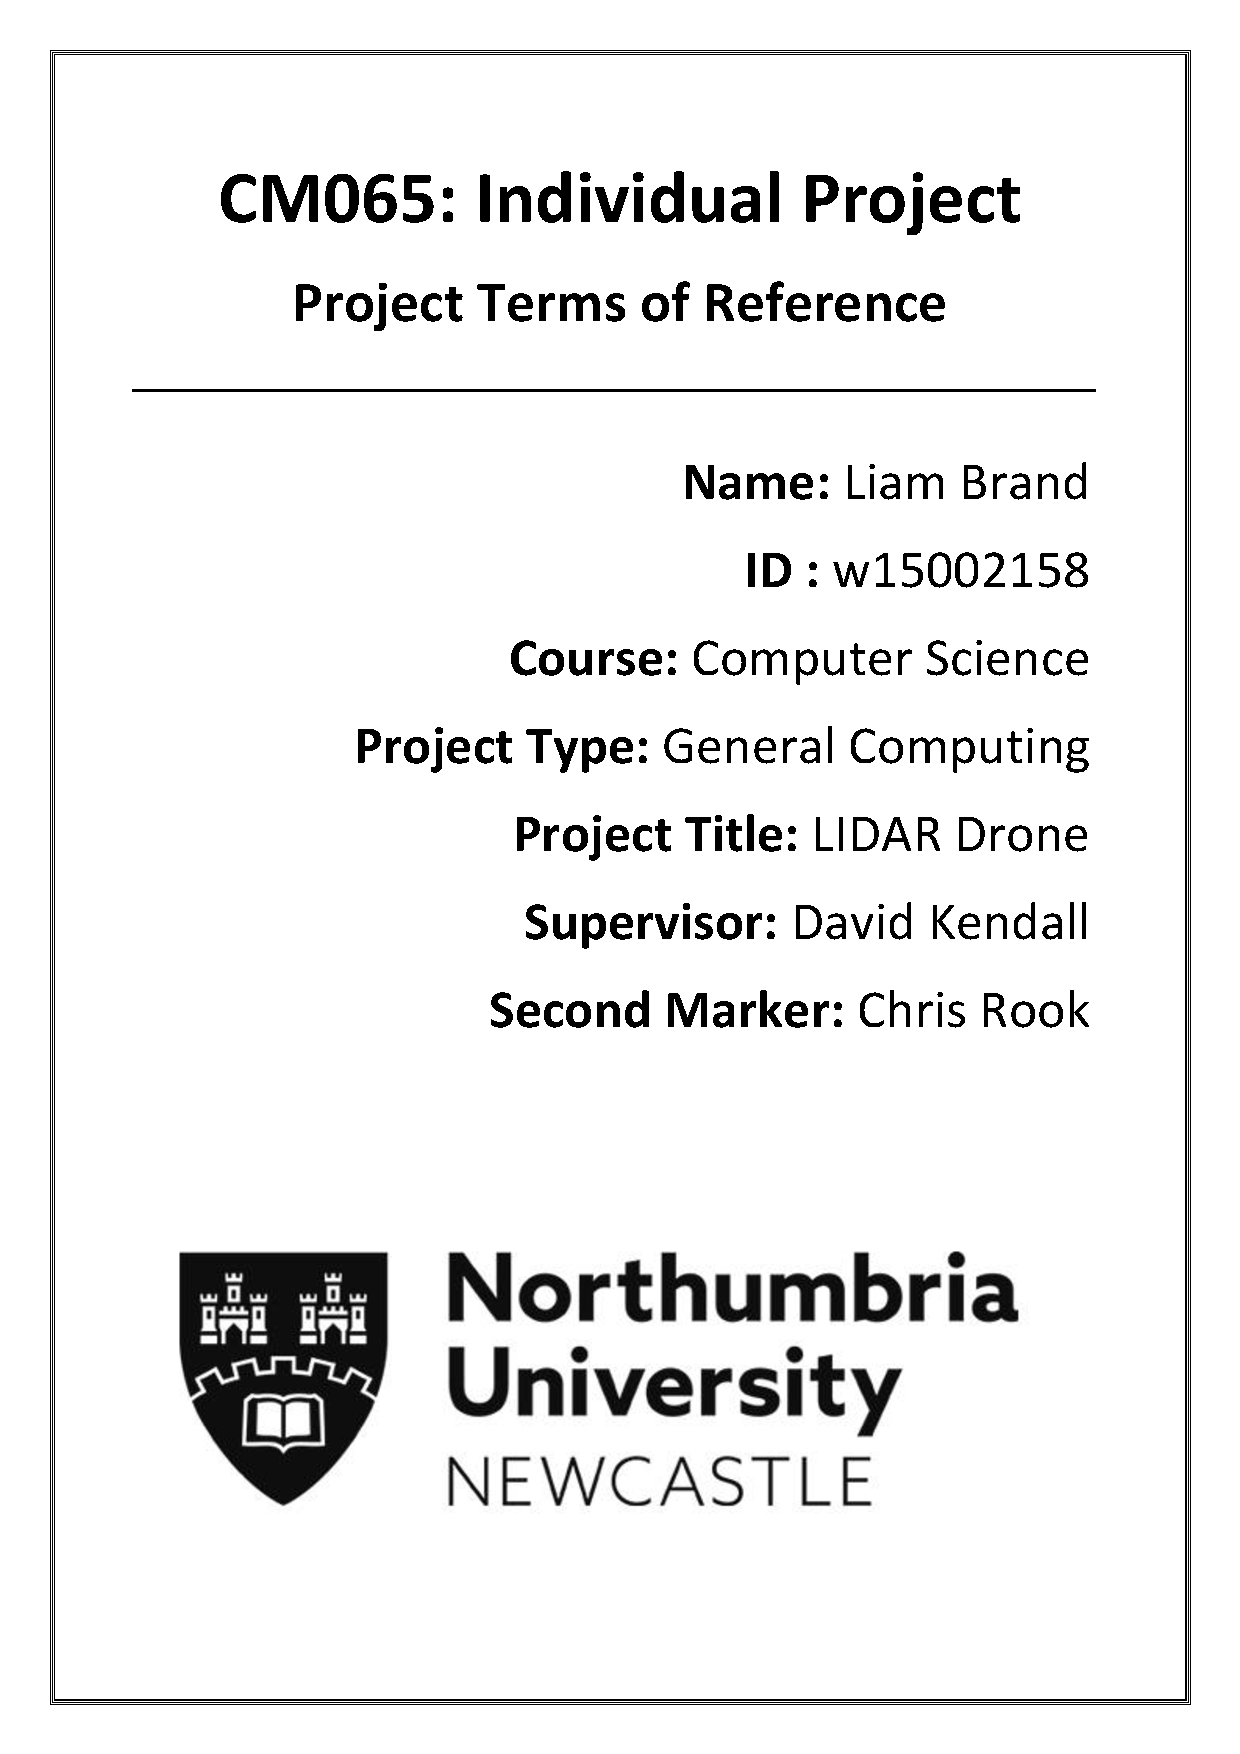
\includepdf[pages=-]{APPENDICES/TOR.pdf}
	\chapter{Program Code}
		\subsection{Robot Software}
			\subsubsection{main.cpp}
			Code repository can be found at: \url{https://github.com/liambrand/lidar-robot}
			\lstinputlisting[caption=main.cpp]{APPENDICES/main.cpp}
		\subsection{GUI}
			\subsubsection{mapgui.py}
			Code repository can be found at: \url{https://github.com/liambrand/robot-map-gui}
			\lstinputlisting[caption=mapgui.py, language=python, showstringspaces=false]{APPENDICES/mapgui.py}
	\chapter{Testing}
	\begin{landscape}
	\label{testingappendices}
		\label{testing:testlogs}
					\begin{table}[h!]
						\centering
						\begin{tabular}{| l | l | l |} 
							\hline
							Printed Direction & Direction Moved In & Test Result  \\ [0.5ex] 
							\hline
							Right & Right & Pass   \\
							Left & Left & Pass   \\ 
							Forward & Forward & Pass   \\ 
							Left & Left & Pass   \\ 
							Right & Right & Pass   \\ 
							Forward & Forward & Pass   \\ 
							Right & Right & Pass   \\ 
							Left & Left & Pass   \\ 
							Backward & Backward & Pass   \\ 
							Forward & Forward & Pass   \\ 
							Backward & Backward & Pass   \\ 
							Left & Left & Pass   \\ 
							Right & Right & Pass   \\ 
							Right & Right & Pass  \\ 
							Backward & Backward & Pass   \\ 
							Forward & Forward & Pass   \\ 
							Forward & Forward & Pass  \\ 
							Backward & Backward & Pass  \\ 
							Right & Right & Pass   \\ 
							Forward & Forward & Pass   \\ 
							Backward & Backward & Pass   \\ [1ex] 
							\hline
						\end{tabular}	
					\caption{Movement Integration Tests}
					\label{table:movementtestsbasic}	
					\end{table}
				
					\begin{table}[h!]
						\centering
						\begin{tabular}{| p{2.5cm} | p{5cm} | p{4cm} | p{3cm} | p{1.5cm} |} 
							\hline
							Test & Test Purpose & Expected Result & Actual Result & Pass/Fail \\ [0.5ex] 
							\hline
							Begin sensor & Determine microcontroller's ability to start LIDAR sensor & Sensor starts spinning & As expected & Pass  \\
							
							Output reading & Determine ability to retrieve data from the LIDAR sensor & Terminal prints scan data & As expected & Pass \\
							 
							Stop sensor & Determine microcontroller's ability to stop LIDAR sensor & Sensor stops spinning & As expected & Pass   \\ [1ex] 
							\hline
						\end{tabular}	
					\caption{LIDAR Integration Tests}	
					\label{table:lidartestbasic}
					\end{table}
				
					\begin{table}[h!]
						\centering
						\begin{tabular}{| p{2.5cm} | p{5cm} | p{4cm} | p{3cm} | p{1.5cm} |} 
							\hline
							Test & Test Purpose & Expected Result & Actual Result & Pass/Fail \\ [0.5ex] 
							\hline
							File Creation & Ensure the robot can create files & File present on Micro SD-Card & As expected & Pass  \\
							
							Basic File Writing & Ensure created file contains data & File shouldn't be empty & As expected & Pass \\
							
							Accurate Data & Ensure written data is what the LIDAR has produced & File's data should match what has been output on the terminal & As expected & Pass \\ 
							
							Intense File Writing & See if the system can cope with writing many thousands of readings & File should contain more data, system task should still finish as normal & As expected & Pass \\
							[1ex] 
							\hline
						\end{tabular}
					\caption{File Writing Integration Tests}
					\label{table:filewritingtests}		
					\end{table}
				
					\begin{table}[h!]
						\centering
						\begin{tabular}{| p{2.5cm} | p{5cm} | p{4cm} | p{3cm} | p{1.5cm} |} 
							\hline
							Test & Test Purpose & Expected Result & Actual Result & Pass/Fail \\ [0.5ex] 
							\hline
							GUI Starts & Ensure the GUI starts properly & GUI will start up after being called from the command line & As expected & Pass  \\
							
							File Readings & Ensure the GUI can process the given file & GUI shouldn't encounter errors processing values from the file & As expected & Pass \\
							
							Basic Map Generated & Ensure a basic map can be generated  & GUI should display a map of the environment the robot mapped & Map was not accurate & Fail \\ 
							
							CSM Map Generated & Ensure the GUI can use CSM to generate a map  & GUI should output a map incorporating multiple scans & No such functionality implemented & Fail \\ [1ex] 
							\hline
						\end{tabular}
						\caption{Mapping Integration Tests}
						\label{table:mappingtests}		
					\end{table}
				
					\centering
					\begin{longtable}{| p{2.5cm} | p{5cm} | p{4cm} | p{4cm} | p{1.5cm} | p{2cm} |} 
						\caption{System Tests}
						\label{systemintergrationtestingtable} \\
						\hline
						Test & Test Purpose & Expected Result & Actual Result & Pass/Fail & Comments \\ [0.5ex] 
						\hline
						Drive Forward & The robot should move forwards during its operation & As expected & The robot moved forwards when it was switched on & Pass & Hardcoded movement  \\
	
						Drive Right & The robot should move right during its operation & The robot is able to move right & The robot couldn't move right & Fail &   \\
							
						Drive Left & The robot should move left during its operation & The robot is able to move left & The robot couldn't move left & Fail &   \\
						
						Obstacle Avoidance & The robot should navigate around obstacles during operation & The robot is able to avoid obstacles & The robot didn't detect obstacles & Fail &   \\
							
						Motor Obstructions & During the previous drive tests, there should be no obstructions to the motors from the robot's other components & As expected & The robot's motors didnt get blocked & Pass &   \\
						
						Power Failured & During the previous drive tests, there should be no power issues & Robot will complete operation without issue & Microcontroller battery's GND cable slips out & Fail &   \\
							
						Scanning & The robot should stop to scan & The robot stops and scans its environment & As predicteda & Pass &   \\ 
							
						Write Scan Data & Ensure the robot can write scanned data to the Micro SD-Card & The Micro SD-Card will contain a file with scan data & As expected & Pass & Plugged in and viewed with USB adapter  \\
							 
						Writing Duration & Ensure the robot writes data to the Micro-SD Card in a reasonable time  & Writing should be done in under ten seconds & As expected & Pass &   \\ 
							
						Generate Map & Using the robot's scan data, the GUI should produce a basic map & Map will be produced resembling the robot's environment & Map was produced but didn't resemble the environment & Fail &  \\ 
							
						Generate Map Without File & Make the GUI attempt to generate a map without an available file & GUI will catch and handle a runtime exception & As expected & Pass &  \\ 
							
						Map Multiple Areas & Mapping should work on multiple different environments & Each map will be accurate to the environment the robot was in & Maps didn't resemble the environment & Fail &  \\ 
							
						Repeated Mapping & Repeated maps of the same area should look similar & Map will be produced resembling the robot's environment & Maps didn't resemble the environment & Fail &  \\ 
							
						SLAM & The system should be capable of producing a dynamic map using multiple scans from different locations & The GUI creates a map from the robot's scan data & No such functionality & Fail &  \\ [1ex] 
							\hline
					\end{longtable}
			\end{landscape}			

		\section{Test Code}
		\label{testing:testcode}
			\subsection{Basic Movement Testing}
			\label{testcode:movementbasic}
			\begin{lstlisting}
while (true) {
	// Random number between 0 and 3
	int r = rand() % 4;
					
	if(r == 0) {
		pc.printf("Forward");
		goForward();
	}
					
	if(r == 1) {
		pc.printf("Right");
		goRight();
	}
					
	if(r == 2) {
		pc.printf("Back");
		goBackward();
	}
					
	if(r == 3) {
		pc.printf("Left");
		goLeft();
	}

	OSTimeDlyHMSM(0,0,3,0);
}
			\end{lstlisting}
			
			\subsection{LIDAR Testing}
			\label{testcode:observation1}
			\begin{lstlisting}
static void appTaskLidarTest(void *pdata) {
	dtr = 0;
	rplidar.begin(lidar_device);
	rplidar.startScan();
	struct RPLidarMeasurement measurement;
				
	while (true) {
		dtr = 1;
		rplidar.waitPoint();
		measurement = rplidar.getCurrentPoint();
		pc.printf("Distance: %f Angle:%f\n", measurement.angle, measurement.distance);
		dtr = 0;
		OSTimeDlyHMSM(0,0,1,0);
	}
}
			\end{lstlisting}
			
			\subsection{SDFileSystem Testing}
			\label{testcode:filewriting2}
			\begin{lstlisting}
dtr = 1;
rplidar.begin(lidar_device);
rplidar.startScan();
struct RPLidarMeasurement measurement;
				
static void writeTest() {
	struct RPLidarMeasurement measurement;

	// Create the readings file on the Micro SD-Card
	FILE *fp = fopen("/sd/readings.txt", "w");
					
	// Log if the file cannot be made
	if (fp == NULL) {
		pc.printf("Unable to access/create file \n");
	}

	for(int i = 0; i < 10; i++) {
		lidar.waitPoint();
		measurement = lidar.getCurrentPoint();
		pc.printf("Angle:%f Distance:%f\n", measurement.angle, measurement.distance);
		fprintf(fp, "%f %f\r\n", measurement.angle, measurement.distance);
	}
					
	// Close file
	fclose(fp);
}
			\end{lstlisting}
	
	\chapter{Hardware Documents}
	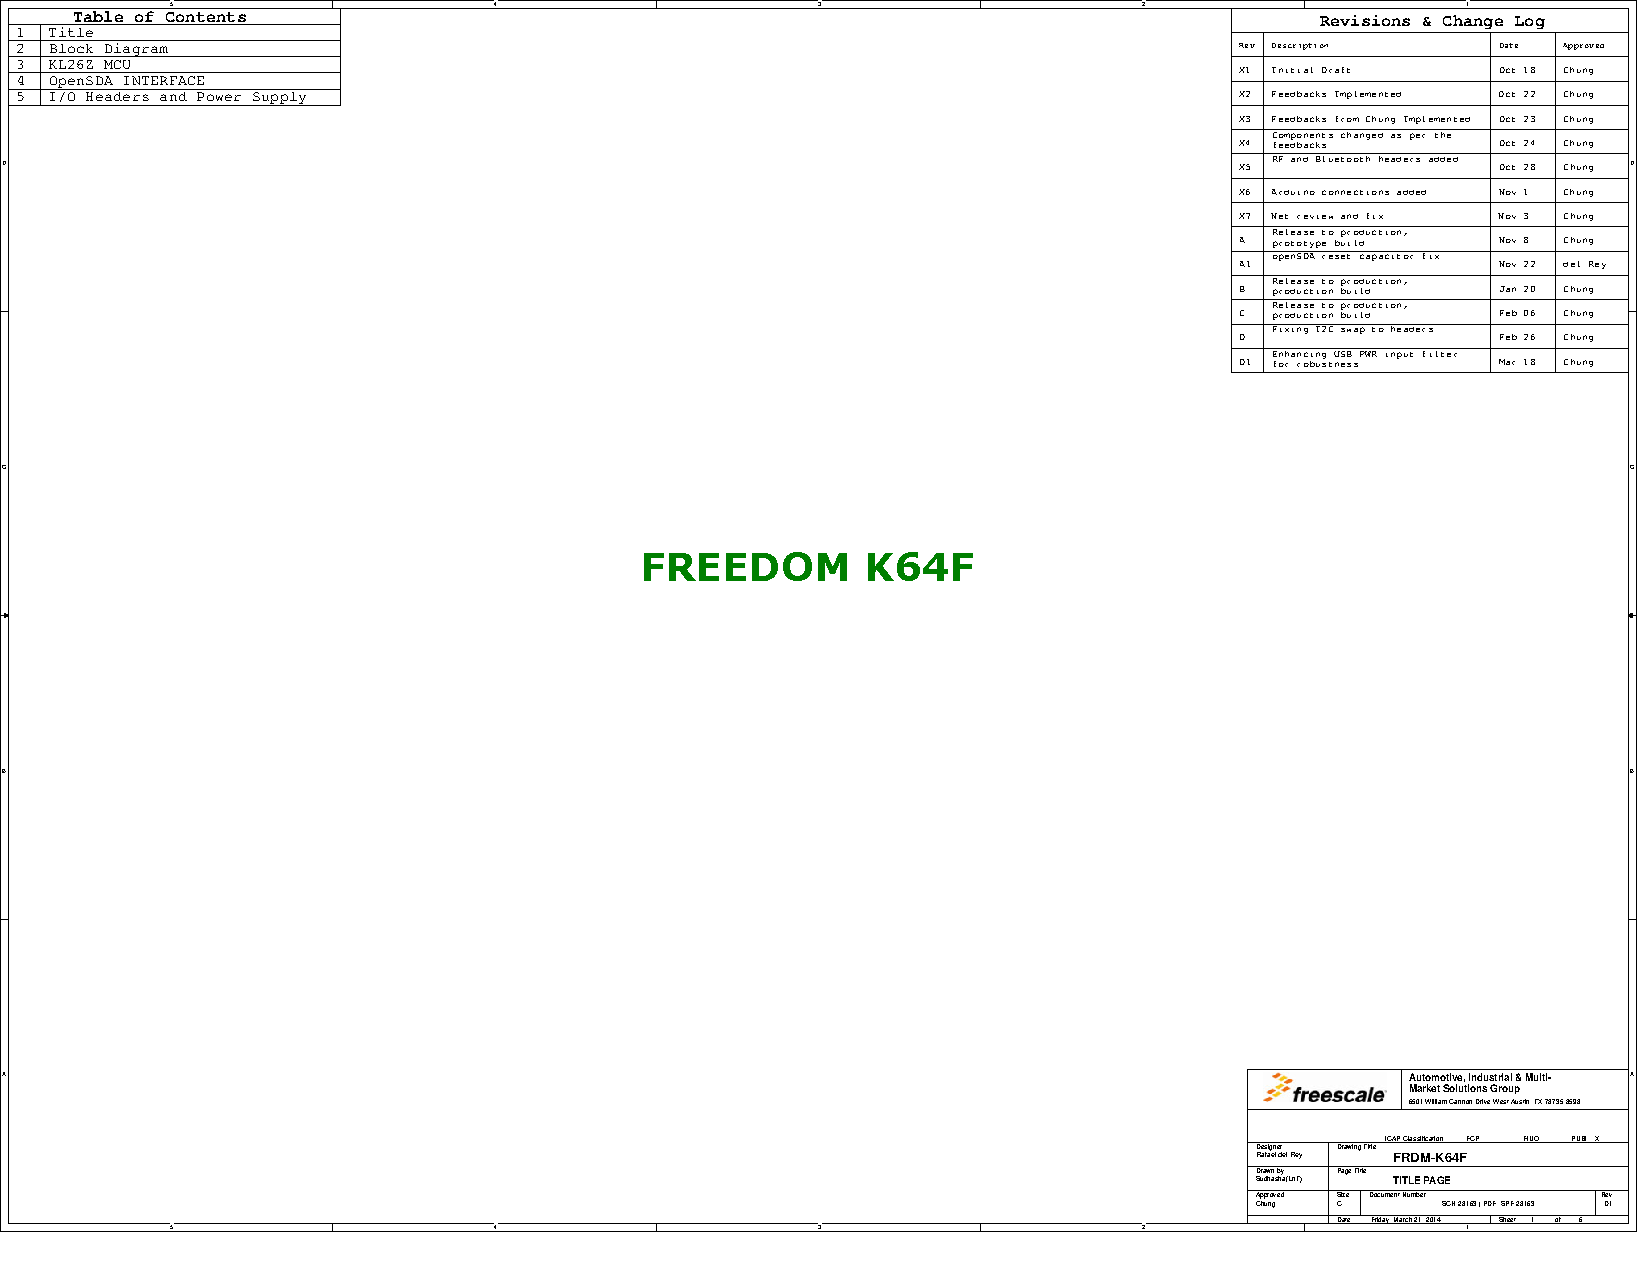
\includepdf[pages=-]{APPENDICES/k64fcircuitdiagram.pdf}
	\chapter{Ethics Form}
	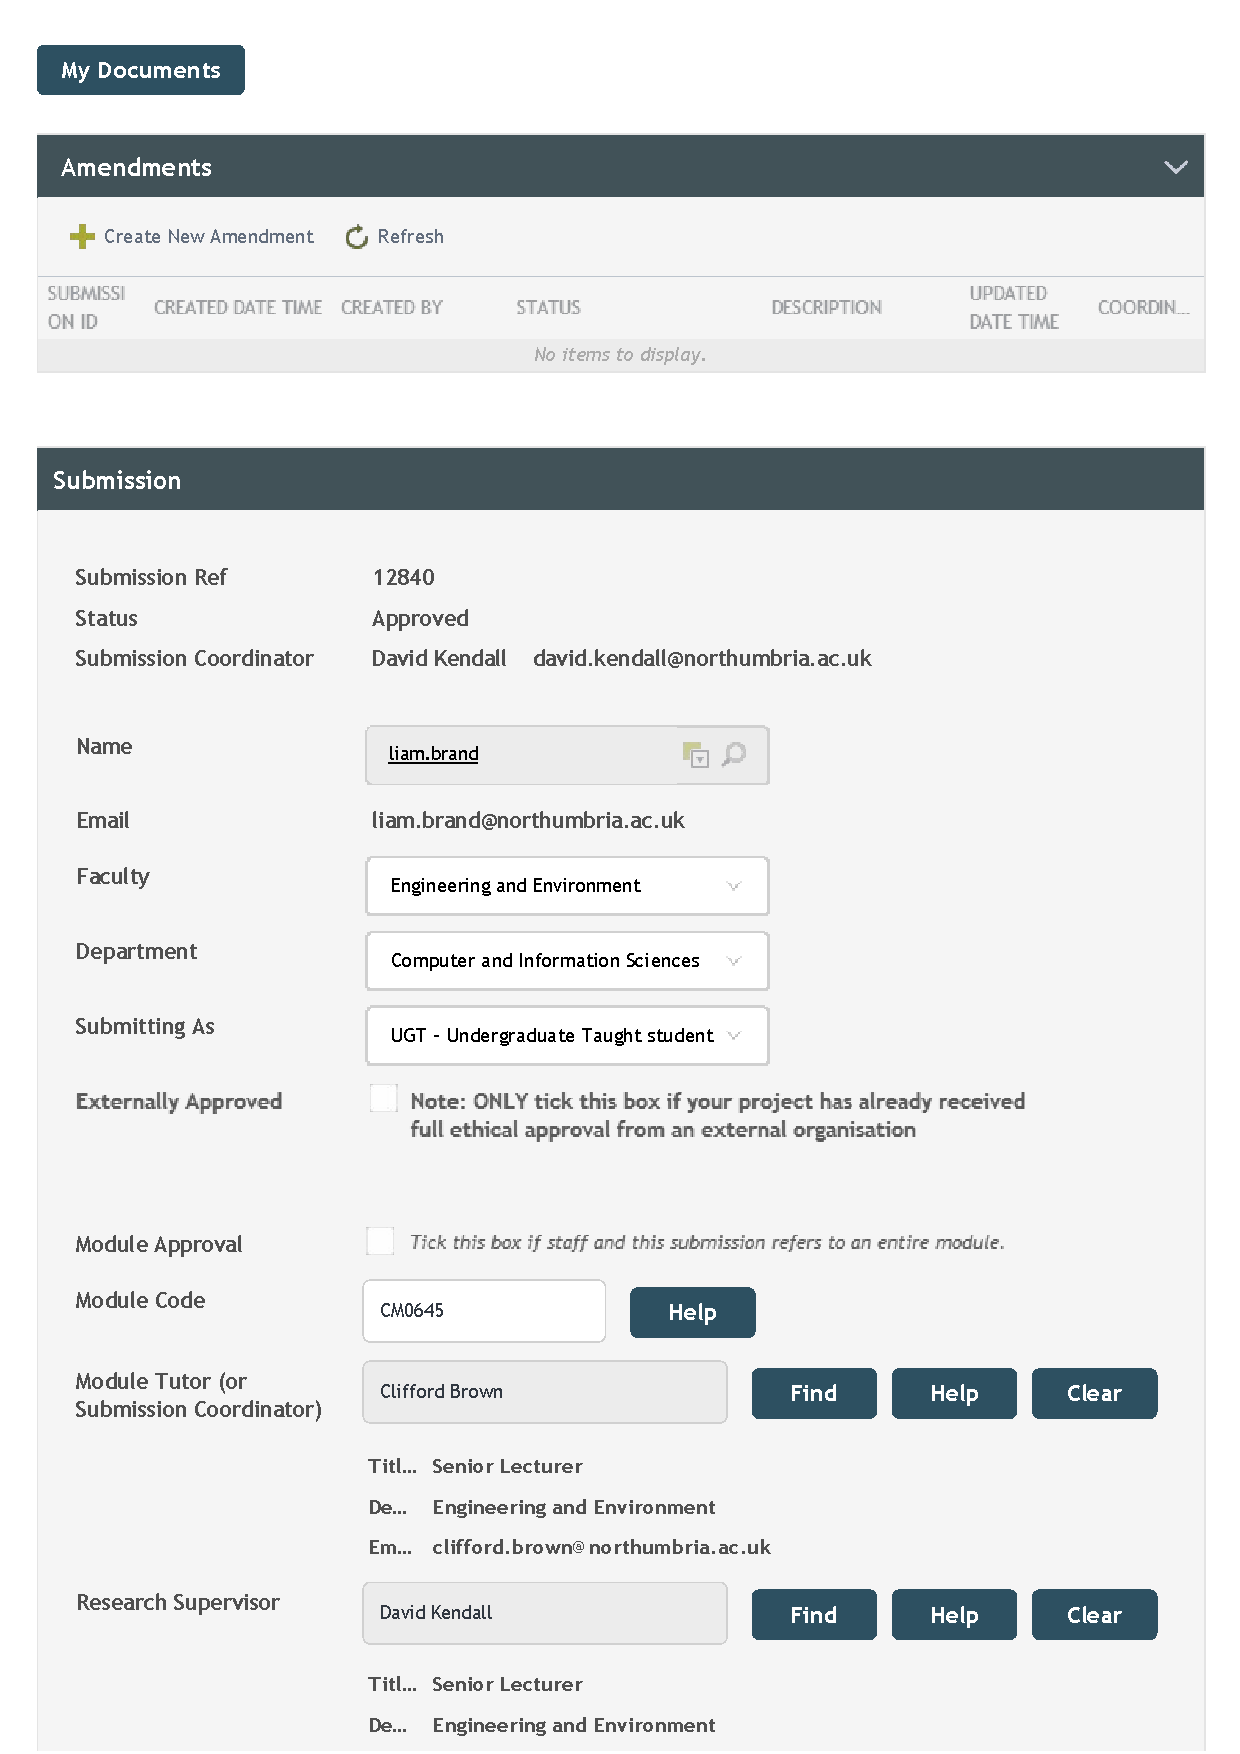
\includepdf[pages=-]{APPENDICES/ethicsonlineform.pdf}
	\end{appendices}
			

	%\appendix
	%\part{Appendices}
	\begin{appendices}
	\chapter{Terms of Reference}
	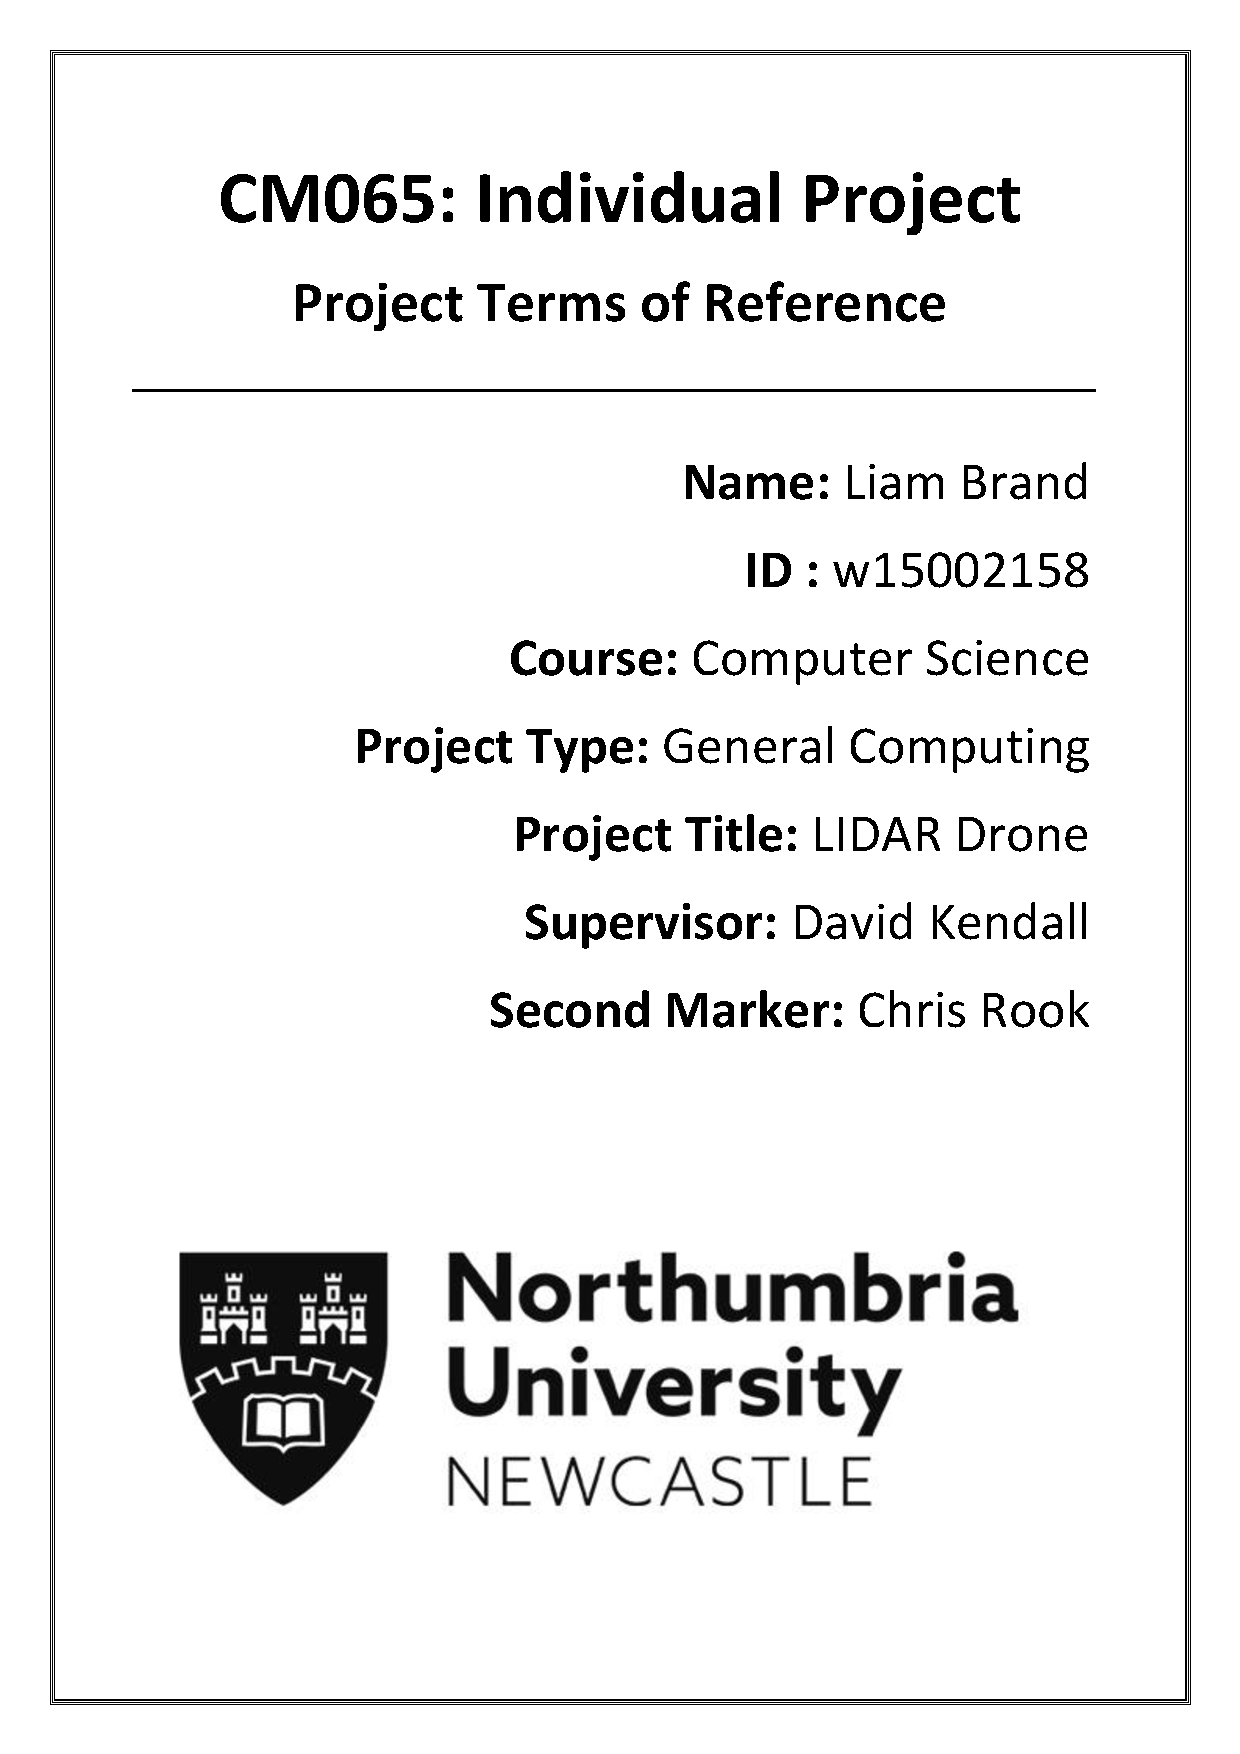
\includepdf[pages=-]{APPENDICES/TOR.pdf}
	\chapter{Program Code}
		\subsection{Robot Software}
			\subsubsection{main.cpp}
			Code repository can be found at: \url{https://github.com/liambrand/lidar-robot}
			\lstinputlisting[caption=main.cpp]{APPENDICES/main.cpp}
		\subsection{GUI}
			\subsubsection{mapgui.py}
			Code repository can be found at: \url{https://github.com/liambrand/robot-map-gui}
			\lstinputlisting[caption=mapgui.py, language=python, showstringspaces=false]{APPENDICES/mapgui.py}
	\chapter{Testing}
	\begin{landscape}
	\label{testingappendices}
		\label{testing:testlogs}
					\begin{table}[h!]
						\centering
						\begin{tabular}{| l | l | l |} 
							\hline
							Printed Direction & Direction Moved In & Test Result  \\ [0.5ex] 
							\hline
							Right & Right & Pass   \\
							Left & Left & Pass   \\ 
							Forward & Forward & Pass   \\ 
							Left & Left & Pass   \\ 
							Right & Right & Pass   \\ 
							Forward & Forward & Pass   \\ 
							Right & Right & Pass   \\ 
							Left & Left & Pass   \\ 
							Backward & Backward & Pass   \\ 
							Forward & Forward & Pass   \\ 
							Backward & Backward & Pass   \\ 
							Left & Left & Pass   \\ 
							Right & Right & Pass   \\ 
							Right & Right & Pass  \\ 
							Backward & Backward & Pass   \\ 
							Forward & Forward & Pass   \\ 
							Forward & Forward & Pass  \\ 
							Backward & Backward & Pass  \\ 
							Right & Right & Pass   \\ 
							Forward & Forward & Pass   \\ 
							Backward & Backward & Pass   \\ [1ex] 
							\hline
						\end{tabular}	
					\caption{Movement Integration Tests}
					\label{table:movementtestsbasic}	
					\end{table}
				
					\begin{table}[h!]
						\centering
						\begin{tabular}{| p{2.5cm} | p{5cm} | p{4cm} | p{3cm} | p{1.5cm} |} 
							\hline
							Test & Test Purpose & Expected Result & Actual Result & Pass/Fail \\ [0.5ex] 
							\hline
							Begin sensor & Determine microcontroller's ability to start LIDAR sensor & Sensor starts spinning & As expected & Pass  \\
							
							Output reading & Determine ability to retrieve data from the LIDAR sensor & Terminal prints scan data & As expected & Pass \\
							 
							Stop sensor & Determine microcontroller's ability to stop LIDAR sensor & Sensor stops spinning & As expected & Pass   \\ [1ex] 
							\hline
						\end{tabular}	
					\caption{LIDAR Integration Tests}	
					\label{table:lidartestbasic}
					\end{table}
				
					\begin{table}[h!]
						\centering
						\begin{tabular}{| p{2.5cm} | p{5cm} | p{4cm} | p{3cm} | p{1.5cm} |} 
							\hline
							Test & Test Purpose & Expected Result & Actual Result & Pass/Fail \\ [0.5ex] 
							\hline
							File Creation & Ensure the robot can create files & File present on Micro SD-Card & As expected & Pass  \\
							
							Basic File Writing & Ensure created file contains data & File shouldn't be empty & As expected & Pass \\
							
							Accurate Data & Ensure written data is what the LIDAR has produced & File's data should match what has been output on the terminal & As expected & Pass \\ 
							
							Intense File Writing & See if the system can cope with writing many thousands of readings & File should contain more data, system task should still finish as normal & As expected & Pass \\
							[1ex] 
							\hline
						\end{tabular}
					\caption{File Writing Integration Tests}
					\label{table:filewritingtests}		
					\end{table}
				
					\begin{table}[h!]
						\centering
						\begin{tabular}{| p{2.5cm} | p{5cm} | p{4cm} | p{3cm} | p{1.5cm} |} 
							\hline
							Test & Test Purpose & Expected Result & Actual Result & Pass/Fail \\ [0.5ex] 
							\hline
							GUI Starts & Ensure the GUI starts properly & GUI will start up after being called from the command line & As expected & Pass  \\
							
							File Readings & Ensure the GUI can process the given file & GUI shouldn't encounter errors processing values from the file & As expected & Pass \\
							
							Basic Map Generated & Ensure a basic map can be generated  & GUI should display a map of the environment the robot mapped & Map was not accurate & Fail \\ 
							
							CSM Map Generated & Ensure the GUI can use CSM to generate a map  & GUI should output a map incorporating multiple scans & No such functionality implemented & Fail \\ [1ex] 
							\hline
						\end{tabular}
						\caption{Mapping Integration Tests}
						\label{table:mappingtests}		
					\end{table}
				
					\centering
					\begin{longtable}{| p{2.5cm} | p{5cm} | p{4cm} | p{4cm} | p{1.5cm} | p{2cm} |} 
						\caption{System Tests}
						\label{systemintergrationtestingtable} \\
						\hline
						Test & Test Purpose & Expected Result & Actual Result & Pass/Fail & Comments \\ [0.5ex] 
						\hline
						Drive Forward & The robot should move forwards during its operation & As expected & The robot moved forwards when it was switched on & Pass & Hardcoded movement  \\
	
						Drive Right & The robot should move right during its operation & The robot is able to move right & The robot couldn't move right & Fail &   \\
							
						Drive Left & The robot should move left during its operation & The robot is able to move left & The robot couldn't move left & Fail &   \\
						
						Obstacle Avoidance & The robot should navigate around obstacles during operation & The robot is able to avoid obstacles & The robot didn't detect obstacles & Fail &   \\
							
						Motor Obstructions & During the previous drive tests, there should be no obstructions to the motors from the robot's other components & As expected & The robot's motors didnt get blocked & Pass &   \\
						
						Power Failured & During the previous drive tests, there should be no power issues & Robot will complete operation without issue & Microcontroller battery's GND cable slips out & Fail &   \\
							
						Scanning & The robot should stop to scan & The robot stops and scans its environment & As predicteda & Pass &   \\ 
							
						Write Scan Data & Ensure the robot can write scanned data to the Micro SD-Card & The Micro SD-Card will contain a file with scan data & As expected & Pass & Plugged in and viewed with USB adapter  \\
							 
						Writing Duration & Ensure the robot writes data to the Micro-SD Card in a reasonable time  & Writing should be done in under ten seconds & As expected & Pass &   \\ 
							
						Generate Map & Using the robot's scan data, the GUI should produce a basic map & Map will be produced resembling the robot's environment & Map was produced but didn't resemble the environment & Fail &  \\ 
							
						Generate Map Without File & Make the GUI attempt to generate a map without an available file & GUI will catch and handle a runtime exception & As expected & Pass &  \\ 
							
						Map Multiple Areas & Mapping should work on multiple different environments & Each map will be accurate to the environment the robot was in & Maps didn't resemble the environment & Fail &  \\ 
							
						Repeated Mapping & Repeated maps of the same area should look similar & Map will be produced resembling the robot's environment & Maps didn't resemble the environment & Fail &  \\ 
							
						SLAM & The system should be capable of producing a dynamic map using multiple scans from different locations & The GUI creates a map from the robot's scan data & No such functionality & Fail &  \\ [1ex] 
							\hline
					\end{longtable}
			\end{landscape}			

		\section{Test Code}
		\label{testing:testcode}
			\subsection{Basic Movement Testing}
			\label{testcode:movementbasic}
			\begin{lstlisting}
while (true) {
	// Random number between 0 and 3
	int r = rand() % 4;
					
	if(r == 0) {
		pc.printf("Forward");
		goForward();
	}
					
	if(r == 1) {
		pc.printf("Right");
		goRight();
	}
					
	if(r == 2) {
		pc.printf("Back");
		goBackward();
	}
					
	if(r == 3) {
		pc.printf("Left");
		goLeft();
	}

	OSTimeDlyHMSM(0,0,3,0);
}
			\end{lstlisting}
			
			\subsection{LIDAR Testing}
			\label{testcode:observation1}
			\begin{lstlisting}
static void appTaskLidarTest(void *pdata) {
	dtr = 0;
	rplidar.begin(lidar_device);
	rplidar.startScan();
	struct RPLidarMeasurement measurement;
				
	while (true) {
		dtr = 1;
		rplidar.waitPoint();
		measurement = rplidar.getCurrentPoint();
		pc.printf("Distance: %f Angle:%f\n", measurement.angle, measurement.distance);
		dtr = 0;
		OSTimeDlyHMSM(0,0,1,0);
	}
}
			\end{lstlisting}
			
			\subsection{SDFileSystem Testing}
			\label{testcode:filewriting2}
			\begin{lstlisting}
dtr = 1;
rplidar.begin(lidar_device);
rplidar.startScan();
struct RPLidarMeasurement measurement;
				
static void writeTest() {
	struct RPLidarMeasurement measurement;

	// Create the readings file on the Micro SD-Card
	FILE *fp = fopen("/sd/readings.txt", "w");
					
	// Log if the file cannot be made
	if (fp == NULL) {
		pc.printf("Unable to access/create file \n");
	}

	for(int i = 0; i < 10; i++) {
		lidar.waitPoint();
		measurement = lidar.getCurrentPoint();
		pc.printf("Angle:%f Distance:%f\n", measurement.angle, measurement.distance);
		fprintf(fp, "%f %f\r\n", measurement.angle, measurement.distance);
	}
					
	// Close file
	fclose(fp);
}
			\end{lstlisting}
	
	\chapter{Hardware Documents}
	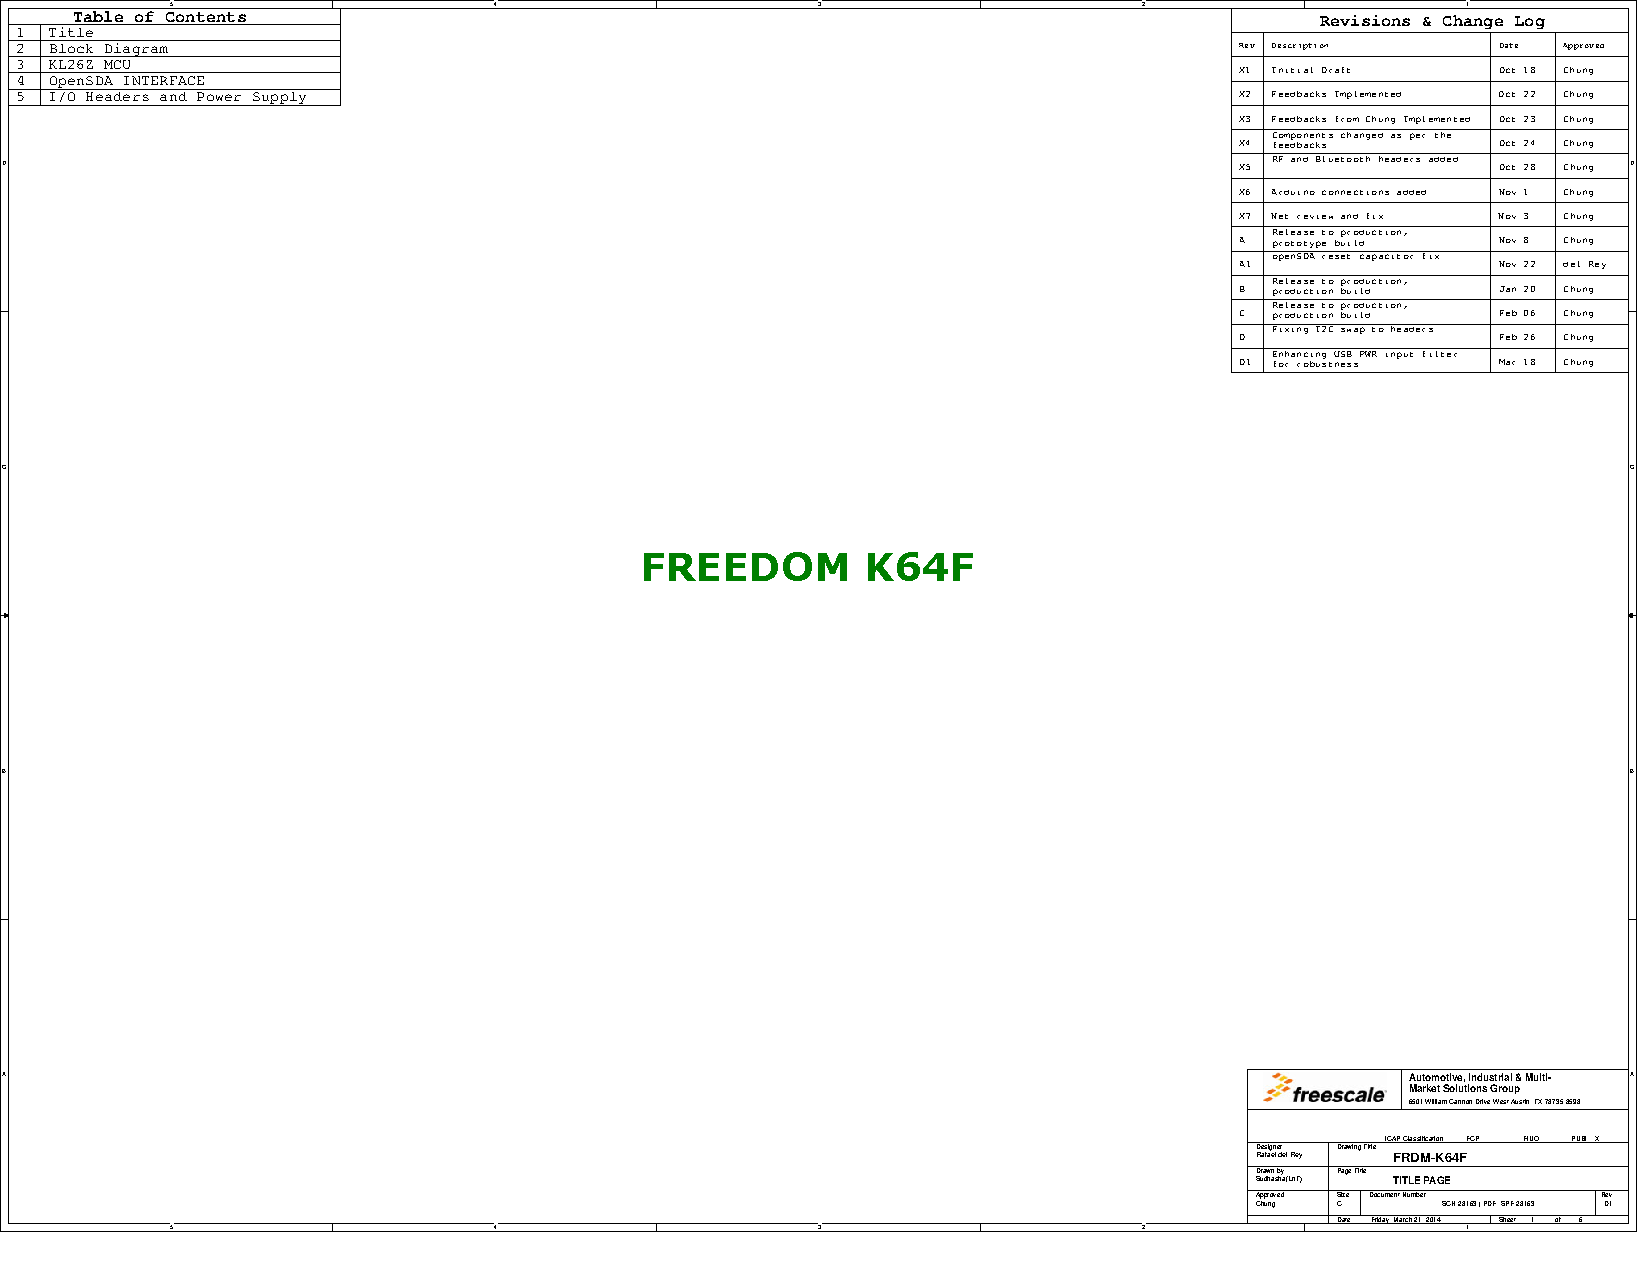
\includepdf[pages=-]{APPENDICES/k64fcircuitdiagram.pdf}
	\chapter{Ethics Form}
	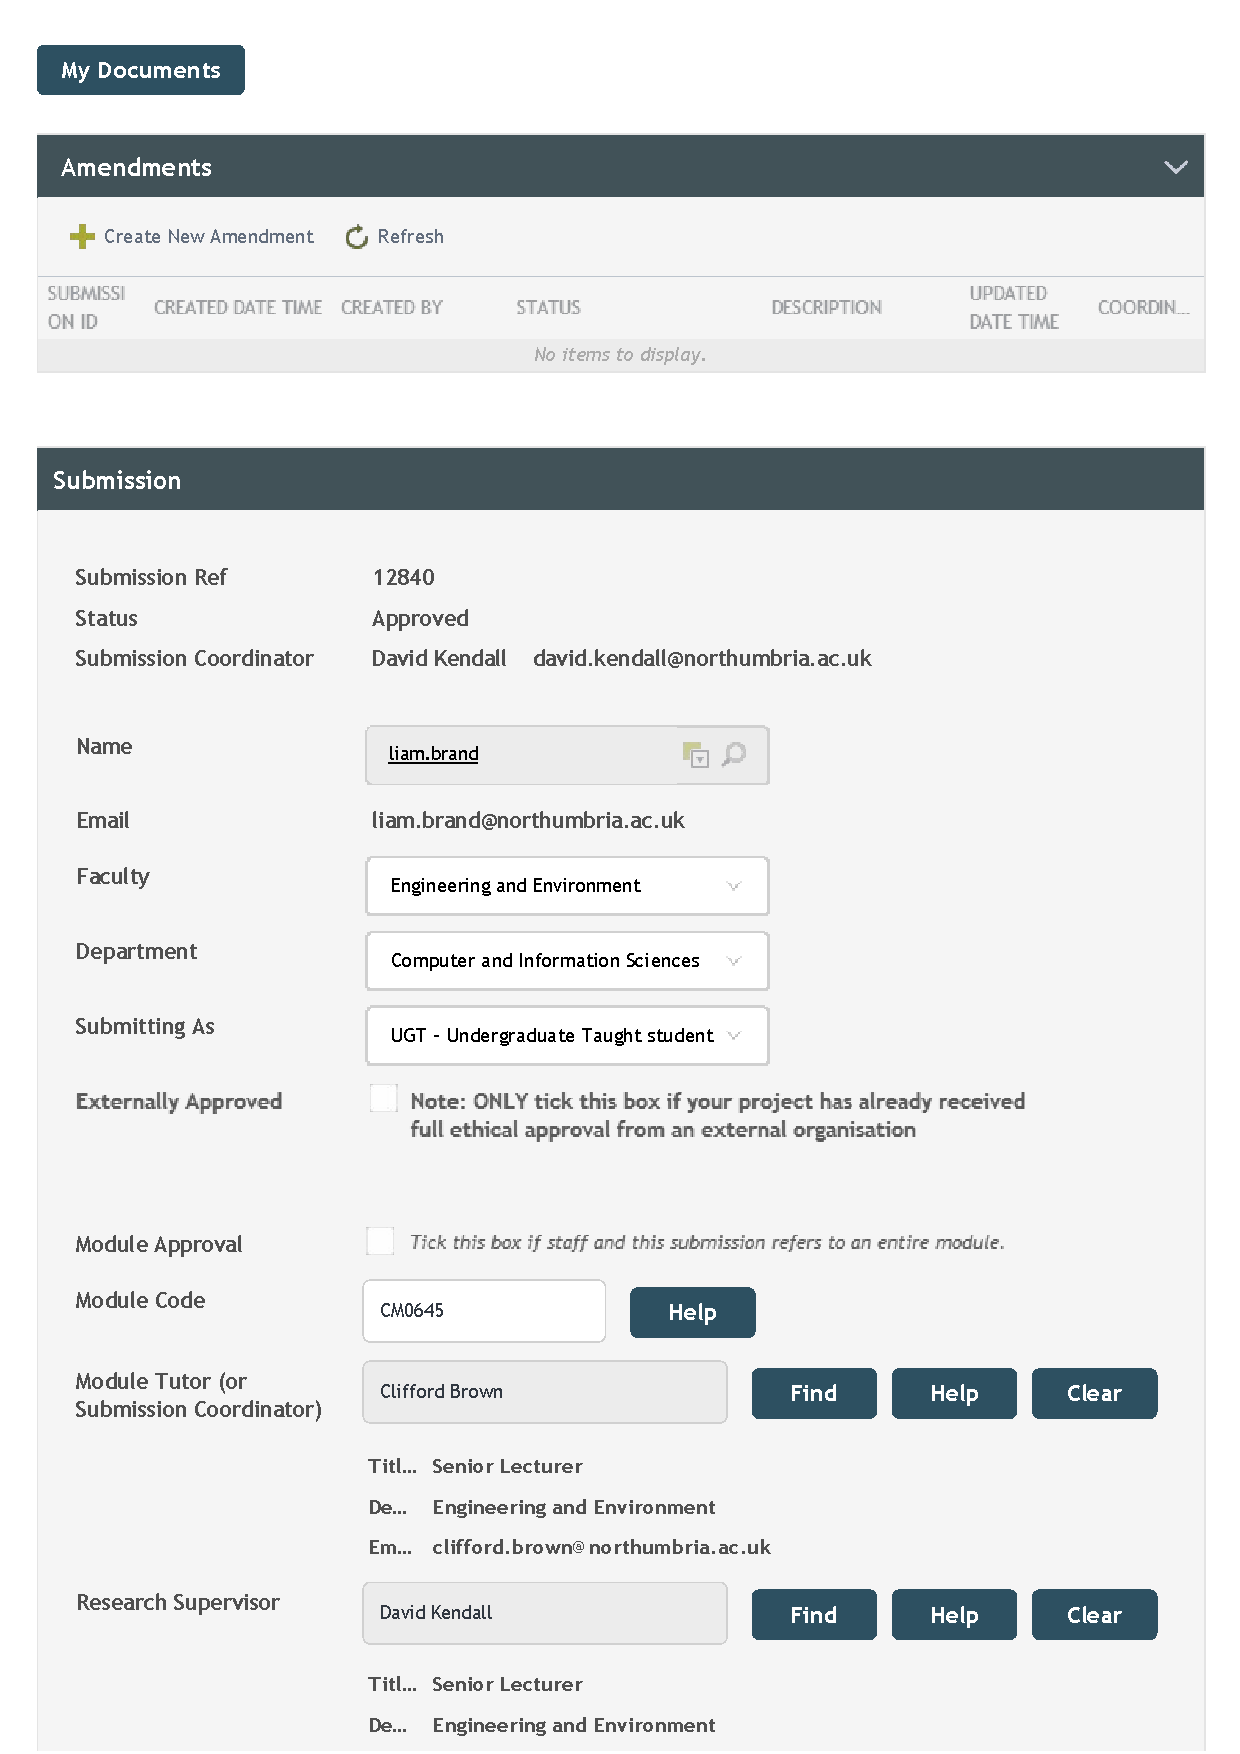
\includepdf[pages=-]{APPENDICES/ethicsonlineform.pdf}
	\end{appendices}
			

	%\part{Appendices}
	\begin{appendices}
	\chapter{Terms of Reference}
	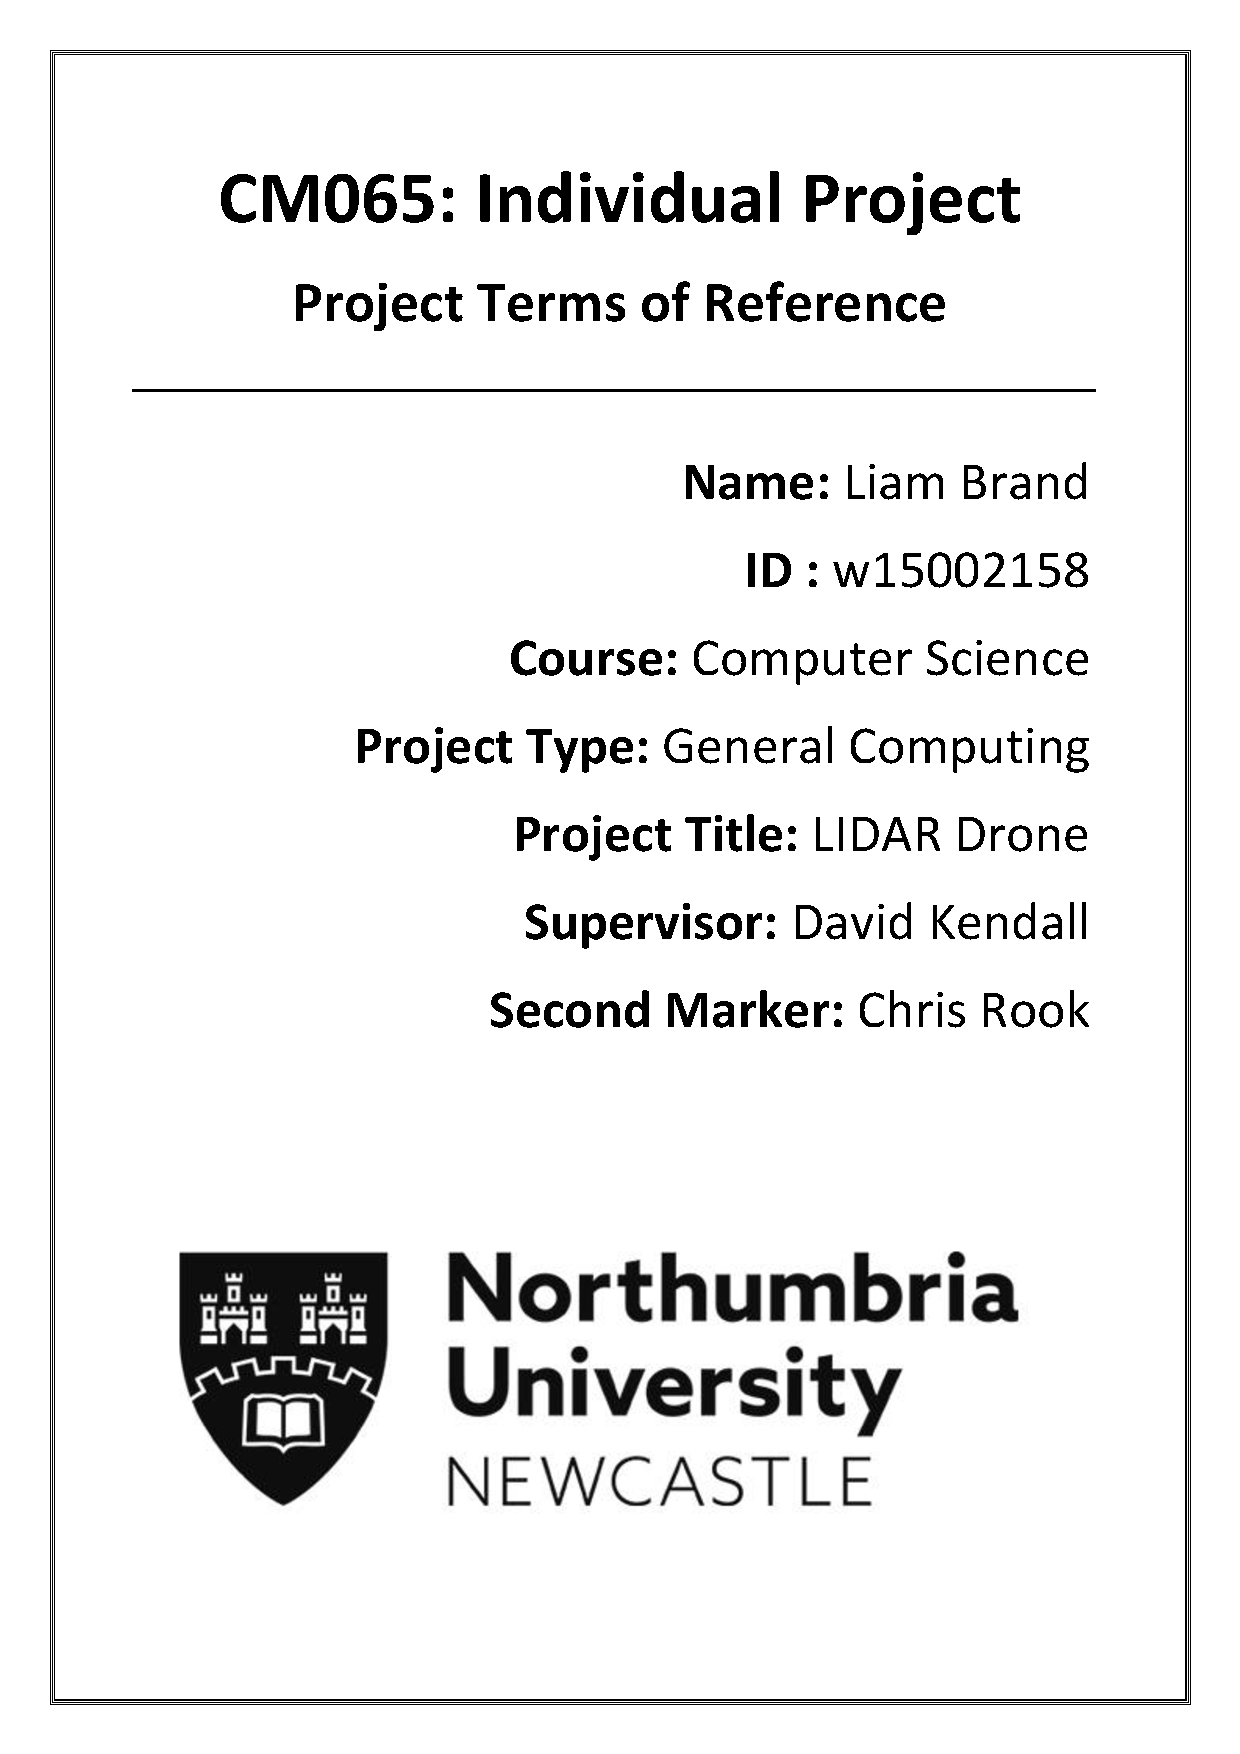
\includepdf[pages=-]{APPENDICES/TOR.pdf}
	\chapter{Program Code}
		\subsection{Robot Software}
			\subsubsection{main.cpp}
			Code repository can be found at: \url{https://github.com/liambrand/lidar-robot}
			\lstinputlisting[caption=main.cpp]{APPENDICES/main.cpp}
		\subsection{GUI}
			\subsubsection{mapgui.py}
			Code repository can be found at: \url{https://github.com/liambrand/robot-map-gui}
			\lstinputlisting[caption=mapgui.py, language=python, showstringspaces=false]{APPENDICES/mapgui.py}
	\chapter{Testing}
	\begin{landscape}
	\label{testingappendices}
		\label{testing:testlogs}
					\begin{table}[h!]
						\centering
						\begin{tabular}{| l | l | l |} 
							\hline
							Printed Direction & Direction Moved In & Test Result  \\ [0.5ex] 
							\hline
							Right & Right & Pass   \\
							Left & Left & Pass   \\ 
							Forward & Forward & Pass   \\ 
							Left & Left & Pass   \\ 
							Right & Right & Pass   \\ 
							Forward & Forward & Pass   \\ 
							Right & Right & Pass   \\ 
							Left & Left & Pass   \\ 
							Backward & Backward & Pass   \\ 
							Forward & Forward & Pass   \\ 
							Backward & Backward & Pass   \\ 
							Left & Left & Pass   \\ 
							Right & Right & Pass   \\ 
							Right & Right & Pass  \\ 
							Backward & Backward & Pass   \\ 
							Forward & Forward & Pass   \\ 
							Forward & Forward & Pass  \\ 
							Backward & Backward & Pass  \\ 
							Right & Right & Pass   \\ 
							Forward & Forward & Pass   \\ 
							Backward & Backward & Pass   \\ [1ex] 
							\hline
						\end{tabular}	
					\caption{Movement Integration Tests}
					\label{table:movementtestsbasic}	
					\end{table}
				
					\begin{table}[h!]
						\centering
						\begin{tabular}{| p{2.5cm} | p{5cm} | p{4cm} | p{3cm} | p{1.5cm} |} 
							\hline
							Test & Test Purpose & Expected Result & Actual Result & Pass/Fail \\ [0.5ex] 
							\hline
							Begin sensor & Determine microcontroller's ability to start LIDAR sensor & Sensor starts spinning & As expected & Pass  \\
							
							Output reading & Determine ability to retrieve data from the LIDAR sensor & Terminal prints scan data & As expected & Pass \\
							 
							Stop sensor & Determine microcontroller's ability to stop LIDAR sensor & Sensor stops spinning & As expected & Pass   \\ [1ex] 
							\hline
						\end{tabular}	
					\caption{LIDAR Integration Tests}	
					\label{table:lidartestbasic}
					\end{table}
				
					\begin{table}[h!]
						\centering
						\begin{tabular}{| p{2.5cm} | p{5cm} | p{4cm} | p{3cm} | p{1.5cm} |} 
							\hline
							Test & Test Purpose & Expected Result & Actual Result & Pass/Fail \\ [0.5ex] 
							\hline
							File Creation & Ensure the robot can create files & File present on Micro SD-Card & As expected & Pass  \\
							
							Basic File Writing & Ensure created file contains data & File shouldn't be empty & As expected & Pass \\
							
							Accurate Data & Ensure written data is what the LIDAR has produced & File's data should match what has been output on the terminal & As expected & Pass \\ 
							
							Intense File Writing & See if the system can cope with writing many thousands of readings & File should contain more data, system task should still finish as normal & As expected & Pass \\
							[1ex] 
							\hline
						\end{tabular}
					\caption{File Writing Integration Tests}
					\label{table:filewritingtests}		
					\end{table}
				
					\begin{table}[h!]
						\centering
						\begin{tabular}{| p{2.5cm} | p{5cm} | p{4cm} | p{3cm} | p{1.5cm} |} 
							\hline
							Test & Test Purpose & Expected Result & Actual Result & Pass/Fail \\ [0.5ex] 
							\hline
							GUI Starts & Ensure the GUI starts properly & GUI will start up after being called from the command line & As expected & Pass  \\
							
							File Readings & Ensure the GUI can process the given file & GUI shouldn't encounter errors processing values from the file & As expected & Pass \\
							
							Basic Map Generated & Ensure a basic map can be generated  & GUI should display a map of the environment the robot mapped & Map was not accurate & Fail \\ 
							
							CSM Map Generated & Ensure the GUI can use CSM to generate a map  & GUI should output a map incorporating multiple scans & No such functionality implemented & Fail \\ [1ex] 
							\hline
						\end{tabular}
						\caption{Mapping Integration Tests}
						\label{table:mappingtests}		
					\end{table}
				
					\centering
					\begin{longtable}{| p{2.5cm} | p{5cm} | p{4cm} | p{4cm} | p{1.5cm} | p{2cm} |} 
						\caption{System Tests}
						\label{systemintergrationtestingtable} \\
						\hline
						Test & Test Purpose & Expected Result & Actual Result & Pass/Fail & Comments \\ [0.5ex] 
						\hline
						Drive Forward & The robot should move forwards during its operation & As expected & The robot moved forwards when it was switched on & Pass & Hardcoded movement  \\
	
						Drive Right & The robot should move right during its operation & The robot is able to move right & The robot couldn't move right & Fail &   \\
							
						Drive Left & The robot should move left during its operation & The robot is able to move left & The robot couldn't move left & Fail &   \\
						
						Obstacle Avoidance & The robot should navigate around obstacles during operation & The robot is able to avoid obstacles & The robot didn't detect obstacles & Fail &   \\
							
						Motor Obstructions & During the previous drive tests, there should be no obstructions to the motors from the robot's other components & As expected & The robot's motors didnt get blocked & Pass &   \\
						
						Power Failured & During the previous drive tests, there should be no power issues & Robot will complete operation without issue & Microcontroller battery's GND cable slips out & Fail &   \\
							
						Scanning & The robot should stop to scan & The robot stops and scans its environment & As predicteda & Pass &   \\ 
							
						Write Scan Data & Ensure the robot can write scanned data to the Micro SD-Card & The Micro SD-Card will contain a file with scan data & As expected & Pass & Plugged in and viewed with USB adapter  \\
							 
						Writing Duration & Ensure the robot writes data to the Micro-SD Card in a reasonable time  & Writing should be done in under ten seconds & As expected & Pass &   \\ 
							
						Generate Map & Using the robot's scan data, the GUI should produce a basic map & Map will be produced resembling the robot's environment & Map was produced but didn't resemble the environment & Fail &  \\ 
							
						Generate Map Without File & Make the GUI attempt to generate a map without an available file & GUI will catch and handle a runtime exception & As expected & Pass &  \\ 
							
						Map Multiple Areas & Mapping should work on multiple different environments & Each map will be accurate to the environment the robot was in & Maps didn't resemble the environment & Fail &  \\ 
							
						Repeated Mapping & Repeated maps of the same area should look similar & Map will be produced resembling the robot's environment & Maps didn't resemble the environment & Fail &  \\ 
							
						SLAM & The system should be capable of producing a dynamic map using multiple scans from different locations & The GUI creates a map from the robot's scan data & No such functionality & Fail &  \\ [1ex] 
							\hline
					\end{longtable}
			\end{landscape}			

		\section{Test Code}
		\label{testing:testcode}
			\subsection{Basic Movement Testing}
			\label{testcode:movementbasic}
			\begin{lstlisting}
while (true) {
	// Random number between 0 and 3
	int r = rand() % 4;
					
	if(r == 0) {
		pc.printf("Forward");
		goForward();
	}
					
	if(r == 1) {
		pc.printf("Right");
		goRight();
	}
					
	if(r == 2) {
		pc.printf("Back");
		goBackward();
	}
					
	if(r == 3) {
		pc.printf("Left");
		goLeft();
	}

	OSTimeDlyHMSM(0,0,3,0);
}
			\end{lstlisting}
			
			\subsection{LIDAR Testing}
			\label{testcode:observation1}
			\begin{lstlisting}
static void appTaskLidarTest(void *pdata) {
	dtr = 0;
	rplidar.begin(lidar_device);
	rplidar.startScan();
	struct RPLidarMeasurement measurement;
				
	while (true) {
		dtr = 1;
		rplidar.waitPoint();
		measurement = rplidar.getCurrentPoint();
		pc.printf("Distance: %f Angle:%f\n", measurement.angle, measurement.distance);
		dtr = 0;
		OSTimeDlyHMSM(0,0,1,0);
	}
}
			\end{lstlisting}
			
			\subsection{SDFileSystem Testing}
			\label{testcode:filewriting2}
			\begin{lstlisting}
dtr = 1;
rplidar.begin(lidar_device);
rplidar.startScan();
struct RPLidarMeasurement measurement;
				
static void writeTest() {
	struct RPLidarMeasurement measurement;

	// Create the readings file on the Micro SD-Card
	FILE *fp = fopen("/sd/readings.txt", "w");
					
	// Log if the file cannot be made
	if (fp == NULL) {
		pc.printf("Unable to access/create file \n");
	}

	for(int i = 0; i < 10; i++) {
		lidar.waitPoint();
		measurement = lidar.getCurrentPoint();
		pc.printf("Angle:%f Distance:%f\n", measurement.angle, measurement.distance);
		fprintf(fp, "%f %f\r\n", measurement.angle, measurement.distance);
	}
					
	// Close file
	fclose(fp);
}
			\end{lstlisting}
	
	\chapter{Hardware Documents}
	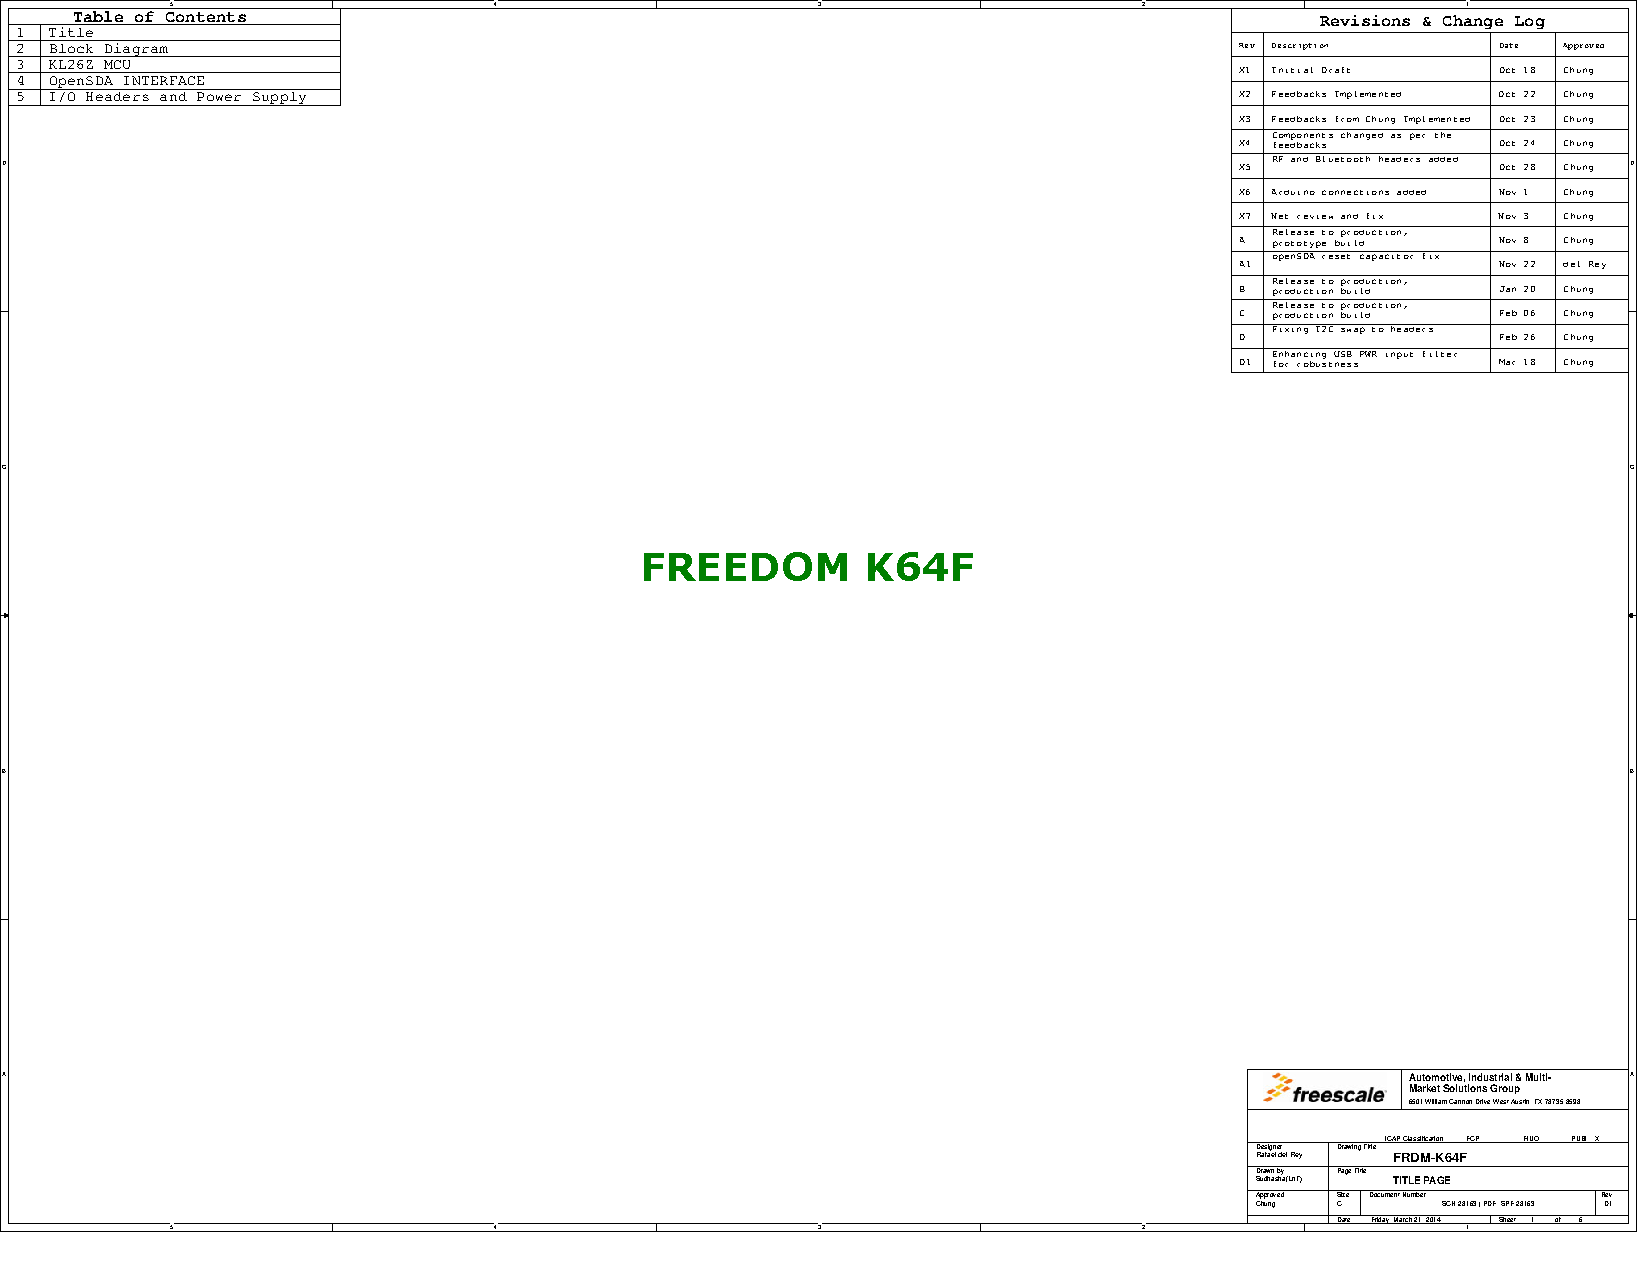
\includepdf[pages=-]{APPENDICES/k64fcircuitdiagram.pdf}
	\chapter{Ethics Form}
	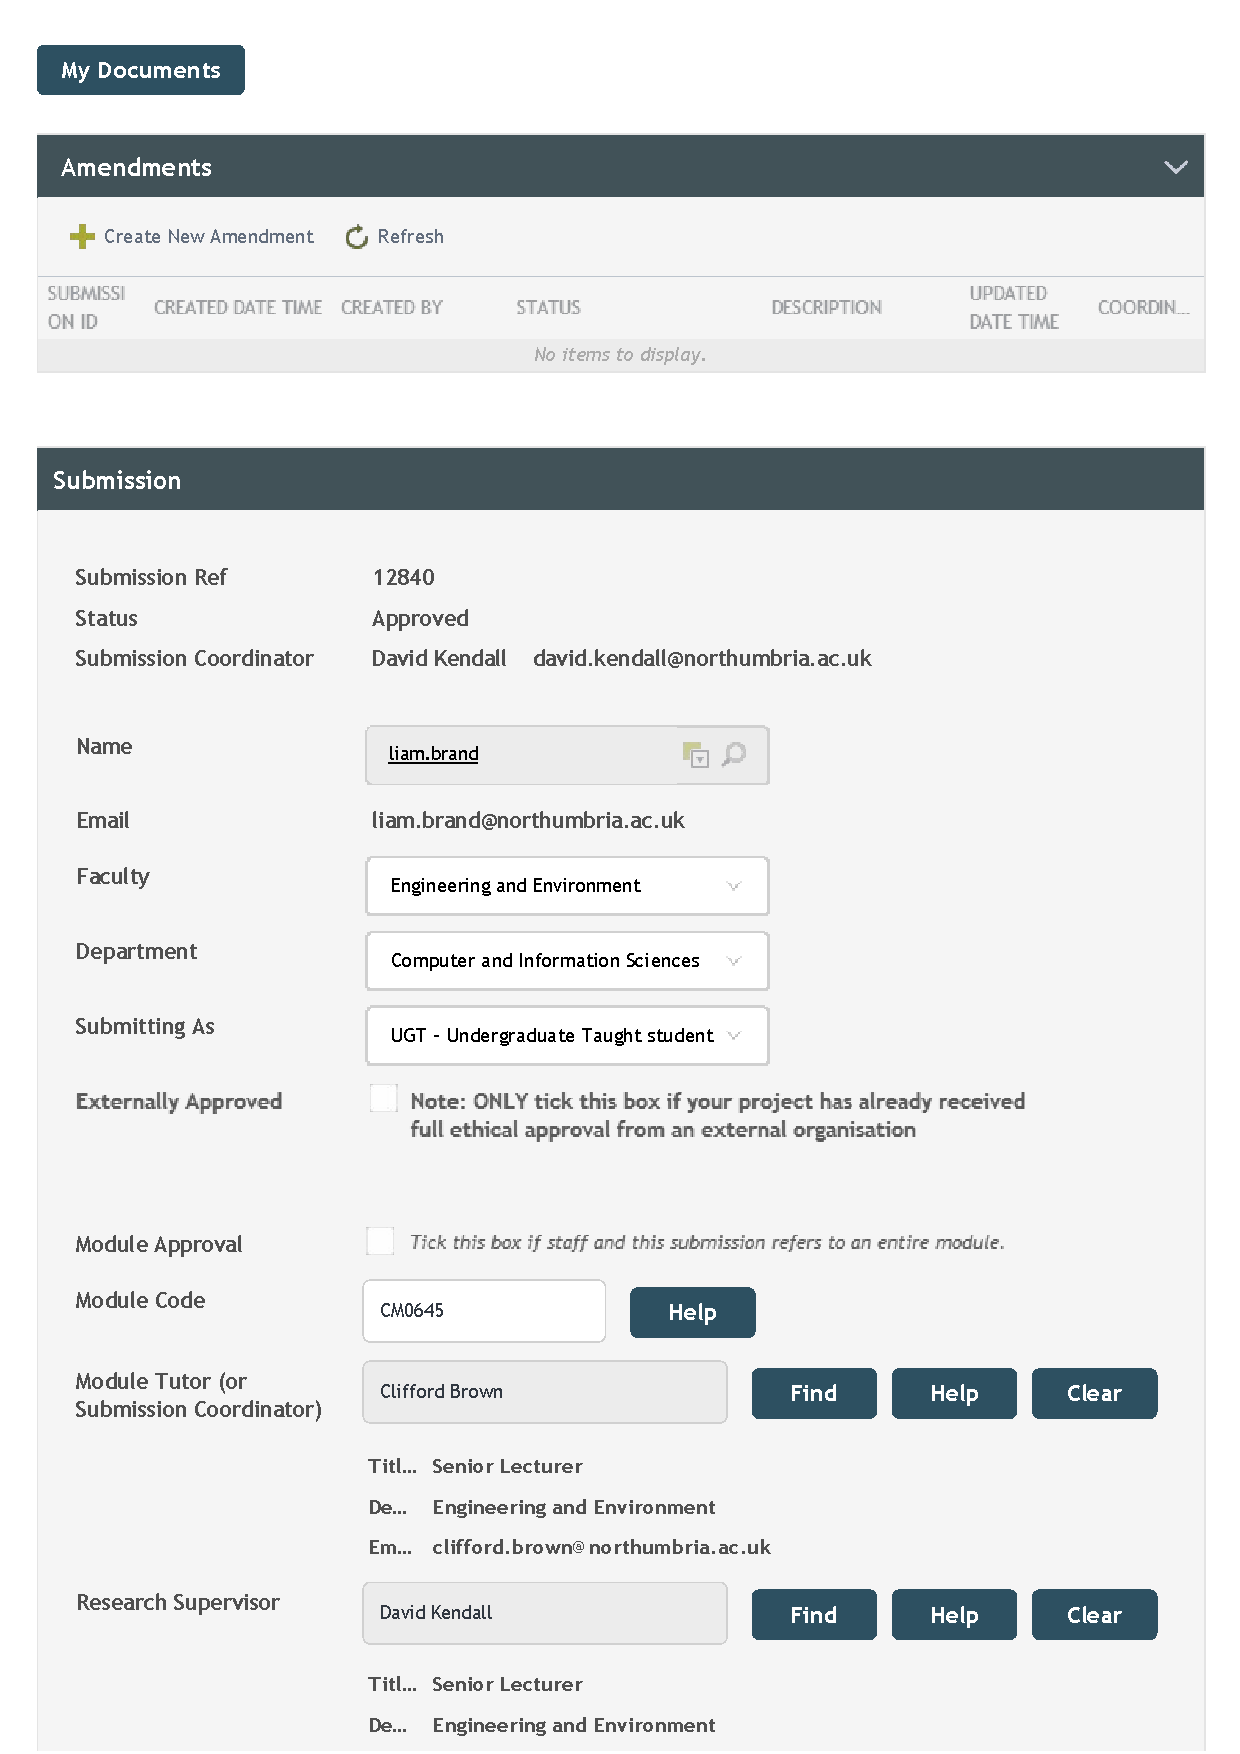
\includepdf[pages=-]{APPENDICES/ethicsonlineform.pdf}
	\end{appendices}
			

	%\part{Appendices}
	\begin{appendices}
	\chapter{Terms of Reference}
	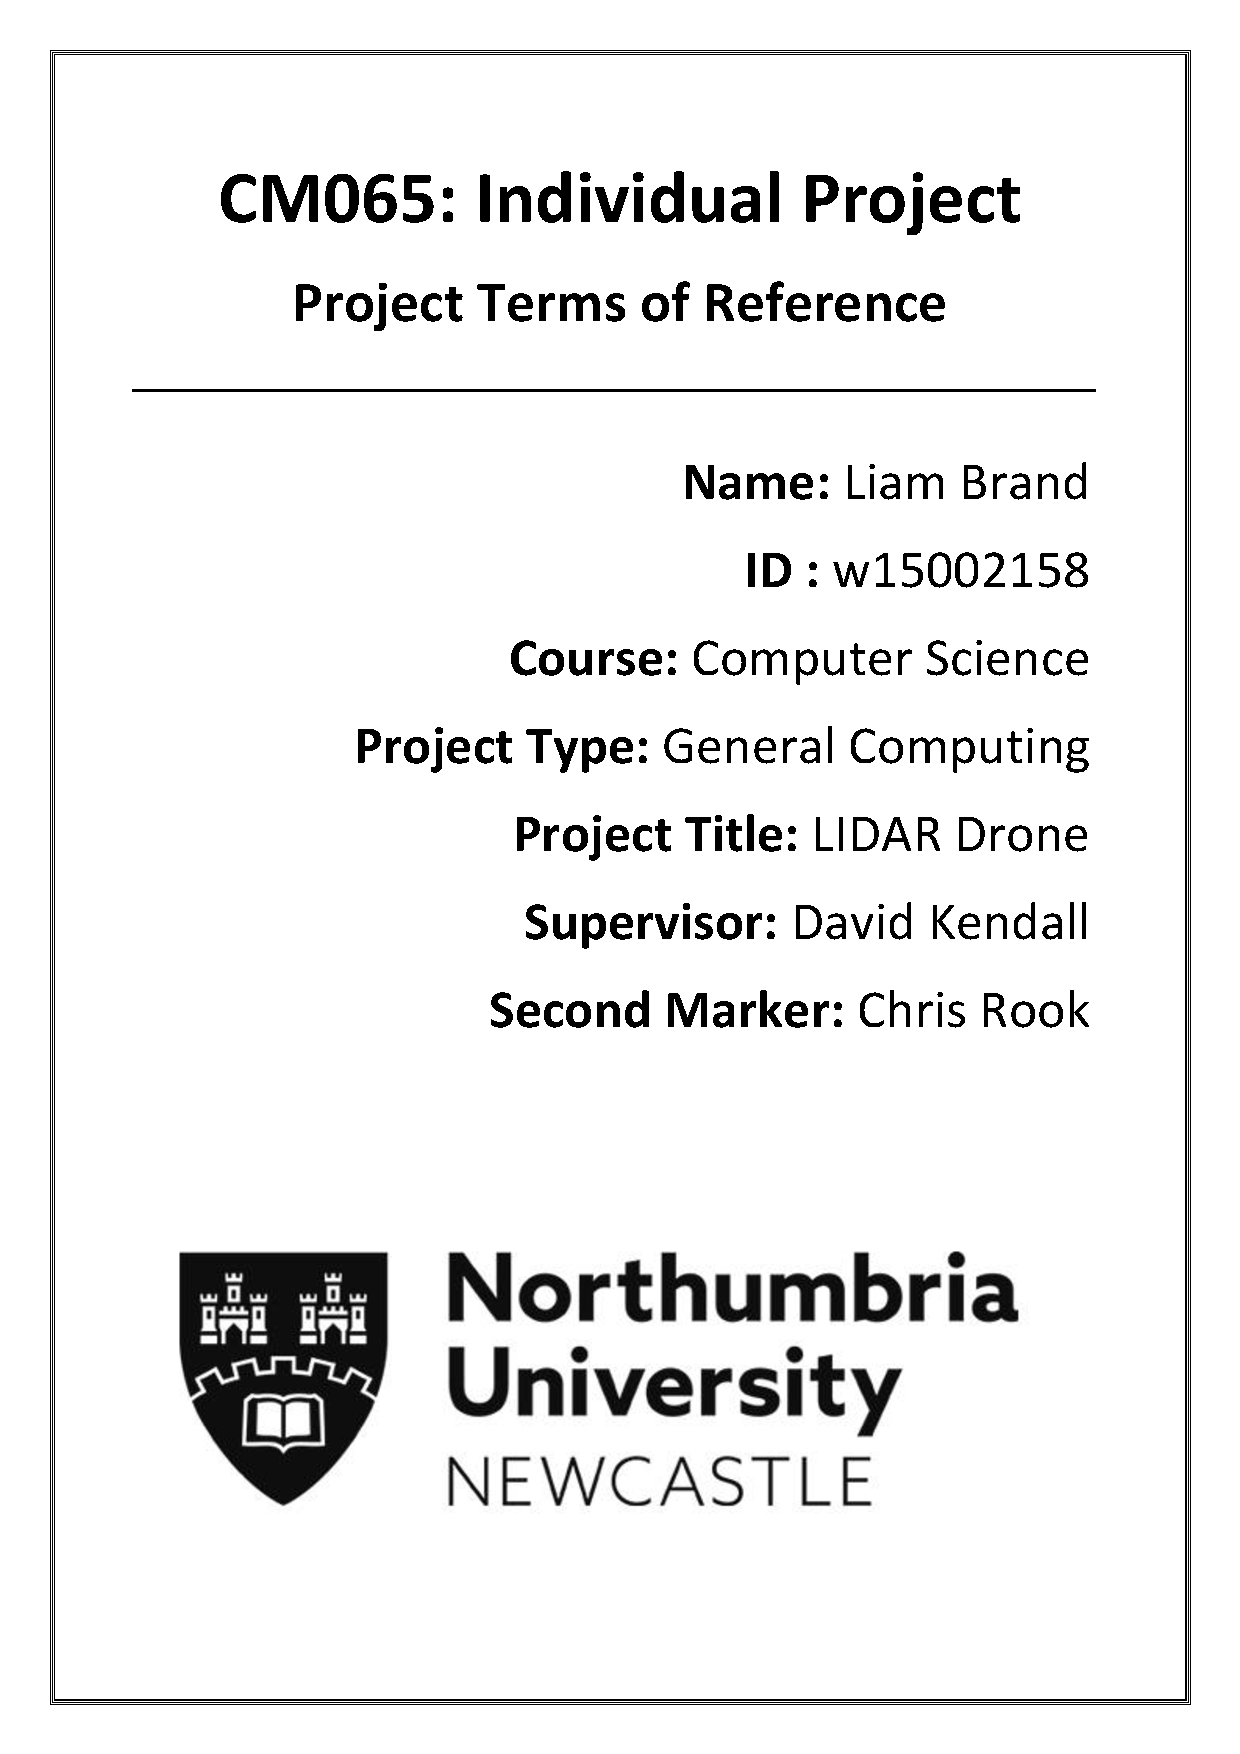
\includepdf[pages=-]{APPENDICES/TOR.pdf}
	\chapter{Program Code}
		\subsection{Robot Software}
			\subsubsection{main.cpp}
			Code repository can be found at: \url{https://github.com/liambrand/lidar-robot}
			\lstinputlisting[caption=main.cpp]{APPENDICES/main.cpp}
		\subsection{GUI}
			\subsubsection{mapgui.py}
			Code repository can be found at: \url{https://github.com/liambrand/robot-map-gui}
			\lstinputlisting[caption=mapgui.py, language=python, showstringspaces=false]{APPENDICES/mapgui.py}
	\chapter{Testing}
	\begin{landscape}
	\label{testingappendices}
		\label{testing:testlogs}
					\begin{table}[h!]
						\centering
						\begin{tabular}{| l | l | l |} 
							\hline
							Printed Direction & Direction Moved In & Test Result  \\ [0.5ex] 
							\hline
							Right & Right & Pass   \\
							Left & Left & Pass   \\ 
							Forward & Forward & Pass   \\ 
							Left & Left & Pass   \\ 
							Right & Right & Pass   \\ 
							Forward & Forward & Pass   \\ 
							Right & Right & Pass   \\ 
							Left & Left & Pass   \\ 
							Backward & Backward & Pass   \\ 
							Forward & Forward & Pass   \\ 
							Backward & Backward & Pass   \\ 
							Left & Left & Pass   \\ 
							Right & Right & Pass   \\ 
							Right & Right & Pass  \\ 
							Backward & Backward & Pass   \\ 
							Forward & Forward & Pass   \\ 
							Forward & Forward & Pass  \\ 
							Backward & Backward & Pass  \\ 
							Right & Right & Pass   \\ 
							Forward & Forward & Pass   \\ 
							Backward & Backward & Pass   \\ [1ex] 
							\hline
						\end{tabular}	
					\caption{Movement Integration Tests}
					\label{table:movementtestsbasic}	
					\end{table}
				
					\begin{table}[h!]
						\centering
						\begin{tabular}{| p{2.5cm} | p{5cm} | p{4cm} | p{3cm} | p{1.5cm} |} 
							\hline
							Test & Test Purpose & Expected Result & Actual Result & Pass/Fail \\ [0.5ex] 
							\hline
							Begin sensor & Determine microcontroller's ability to start LIDAR sensor & Sensor starts spinning & As expected & Pass  \\
							
							Output reading & Determine ability to retrieve data from the LIDAR sensor & Terminal prints scan data & As expected & Pass \\
							 
							Stop sensor & Determine microcontroller's ability to stop LIDAR sensor & Sensor stops spinning & As expected & Pass   \\ [1ex] 
							\hline
						\end{tabular}	
					\caption{LIDAR Integration Tests}	
					\label{table:lidartestbasic}
					\end{table}
				
					\begin{table}[h!]
						\centering
						\begin{tabular}{| p{2.5cm} | p{5cm} | p{4cm} | p{3cm} | p{1.5cm} |} 
							\hline
							Test & Test Purpose & Expected Result & Actual Result & Pass/Fail \\ [0.5ex] 
							\hline
							File Creation & Ensure the robot can create files & File present on Micro SD-Card & As expected & Pass  \\
							
							Basic File Writing & Ensure created file contains data & File shouldn't be empty & As expected & Pass \\
							
							Accurate Data & Ensure written data is what the LIDAR has produced & File's data should match what has been output on the terminal & As expected & Pass \\ 
							
							Intense File Writing & See if the system can cope with writing many thousands of readings & File should contain more data, system task should still finish as normal & As expected & Pass \\
							[1ex] 
							\hline
						\end{tabular}
					\caption{File Writing Integration Tests}
					\label{table:filewritingtests}		
					\end{table}
				
					\begin{table}[h!]
						\centering
						\begin{tabular}{| p{2.5cm} | p{5cm} | p{4cm} | p{3cm} | p{1.5cm} |} 
							\hline
							Test & Test Purpose & Expected Result & Actual Result & Pass/Fail \\ [0.5ex] 
							\hline
							GUI Starts & Ensure the GUI starts properly & GUI will start up after being called from the command line & As expected & Pass  \\
							
							File Readings & Ensure the GUI can process the given file & GUI shouldn't encounter errors processing values from the file & As expected & Pass \\
							
							Basic Map Generated & Ensure a basic map can be generated  & GUI should display a map of the environment the robot mapped & Map was not accurate & Fail \\ 
							
							CSM Map Generated & Ensure the GUI can use CSM to generate a map  & GUI should output a map incorporating multiple scans & No such functionality implemented & Fail \\ [1ex] 
							\hline
						\end{tabular}
						\caption{Mapping Integration Tests}
						\label{table:mappingtests}		
					\end{table}
				
					\centering
					\begin{longtable}{| p{2.5cm} | p{5cm} | p{4cm} | p{4cm} | p{1.5cm} | p{2cm} |} 
						\caption{System Tests}
						\label{systemintergrationtestingtable} \\
						\hline
						Test & Test Purpose & Expected Result & Actual Result & Pass/Fail & Comments \\ [0.5ex] 
						\hline
						Drive Forward & The robot should move forwards during its operation & As expected & The robot moved forwards when it was switched on & Pass & Hardcoded movement  \\
	
						Drive Right & The robot should move right during its operation & The robot is able to move right & The robot couldn't move right & Fail &   \\
							
						Drive Left & The robot should move left during its operation & The robot is able to move left & The robot couldn't move left & Fail &   \\
						
						Obstacle Avoidance & The robot should navigate around obstacles during operation & The robot is able to avoid obstacles & The robot didn't detect obstacles & Fail &   \\
							
						Motor Obstructions & During the previous drive tests, there should be no obstructions to the motors from the robot's other components & As expected & The robot's motors didnt get blocked & Pass &   \\
						
						Power Failured & During the previous drive tests, there should be no power issues & Robot will complete operation without issue & Microcontroller battery's GND cable slips out & Fail &   \\
							
						Scanning & The robot should stop to scan & The robot stops and scans its environment & As predicteda & Pass &   \\ 
							
						Write Scan Data & Ensure the robot can write scanned data to the Micro SD-Card & The Micro SD-Card will contain a file with scan data & As expected & Pass & Plugged in and viewed with USB adapter  \\
							 
						Writing Duration & Ensure the robot writes data to the Micro-SD Card in a reasonable time  & Writing should be done in under ten seconds & As expected & Pass &   \\ 
							
						Generate Map & Using the robot's scan data, the GUI should produce a basic map & Map will be produced resembling the robot's environment & Map was produced but didn't resemble the environment & Fail &  \\ 
							
						Generate Map Without File & Make the GUI attempt to generate a map without an available file & GUI will catch and handle a runtime exception & As expected & Pass &  \\ 
							
						Map Multiple Areas & Mapping should work on multiple different environments & Each map will be accurate to the environment the robot was in & Maps didn't resemble the environment & Fail &  \\ 
							
						Repeated Mapping & Repeated maps of the same area should look similar & Map will be produced resembling the robot's environment & Maps didn't resemble the environment & Fail &  \\ 
							
						SLAM & The system should be capable of producing a dynamic map using multiple scans from different locations & The GUI creates a map from the robot's scan data & No such functionality & Fail &  \\ [1ex] 
							\hline
					\end{longtable}
			\end{landscape}			

		\section{Test Code}
		\label{testing:testcode}
			\subsection{Basic Movement Testing}
			\label{testcode:movementbasic}
			\begin{lstlisting}
while (true) {
	// Random number between 0 and 3
	int r = rand() % 4;
					
	if(r == 0) {
		pc.printf("Forward");
		goForward();
	}
					
	if(r == 1) {
		pc.printf("Right");
		goRight();
	}
					
	if(r == 2) {
		pc.printf("Back");
		goBackward();
	}
					
	if(r == 3) {
		pc.printf("Left");
		goLeft();
	}

	OSTimeDlyHMSM(0,0,3,0);
}
			\end{lstlisting}
			
			\subsection{LIDAR Testing}
			\label{testcode:observation1}
			\begin{lstlisting}
static void appTaskLidarTest(void *pdata) {
	dtr = 0;
	rplidar.begin(lidar_device);
	rplidar.startScan();
	struct RPLidarMeasurement measurement;
				
	while (true) {
		dtr = 1;
		rplidar.waitPoint();
		measurement = rplidar.getCurrentPoint();
		pc.printf("Distance: %f Angle:%f\n", measurement.angle, measurement.distance);
		dtr = 0;
		OSTimeDlyHMSM(0,0,1,0);
	}
}
			\end{lstlisting}
			
			\subsection{SDFileSystem Testing}
			\label{testcode:filewriting2}
			\begin{lstlisting}
dtr = 1;
rplidar.begin(lidar_device);
rplidar.startScan();
struct RPLidarMeasurement measurement;
				
static void writeTest() {
	struct RPLidarMeasurement measurement;

	// Create the readings file on the Micro SD-Card
	FILE *fp = fopen("/sd/readings.txt", "w");
					
	// Log if the file cannot be made
	if (fp == NULL) {
		pc.printf("Unable to access/create file \n");
	}

	for(int i = 0; i < 10; i++) {
		lidar.waitPoint();
		measurement = lidar.getCurrentPoint();
		pc.printf("Angle:%f Distance:%f\n", measurement.angle, measurement.distance);
		fprintf(fp, "%f %f\r\n", measurement.angle, measurement.distance);
	}
					
	// Close file
	fclose(fp);
}
			\end{lstlisting}
	
	\chapter{Hardware Documents}
	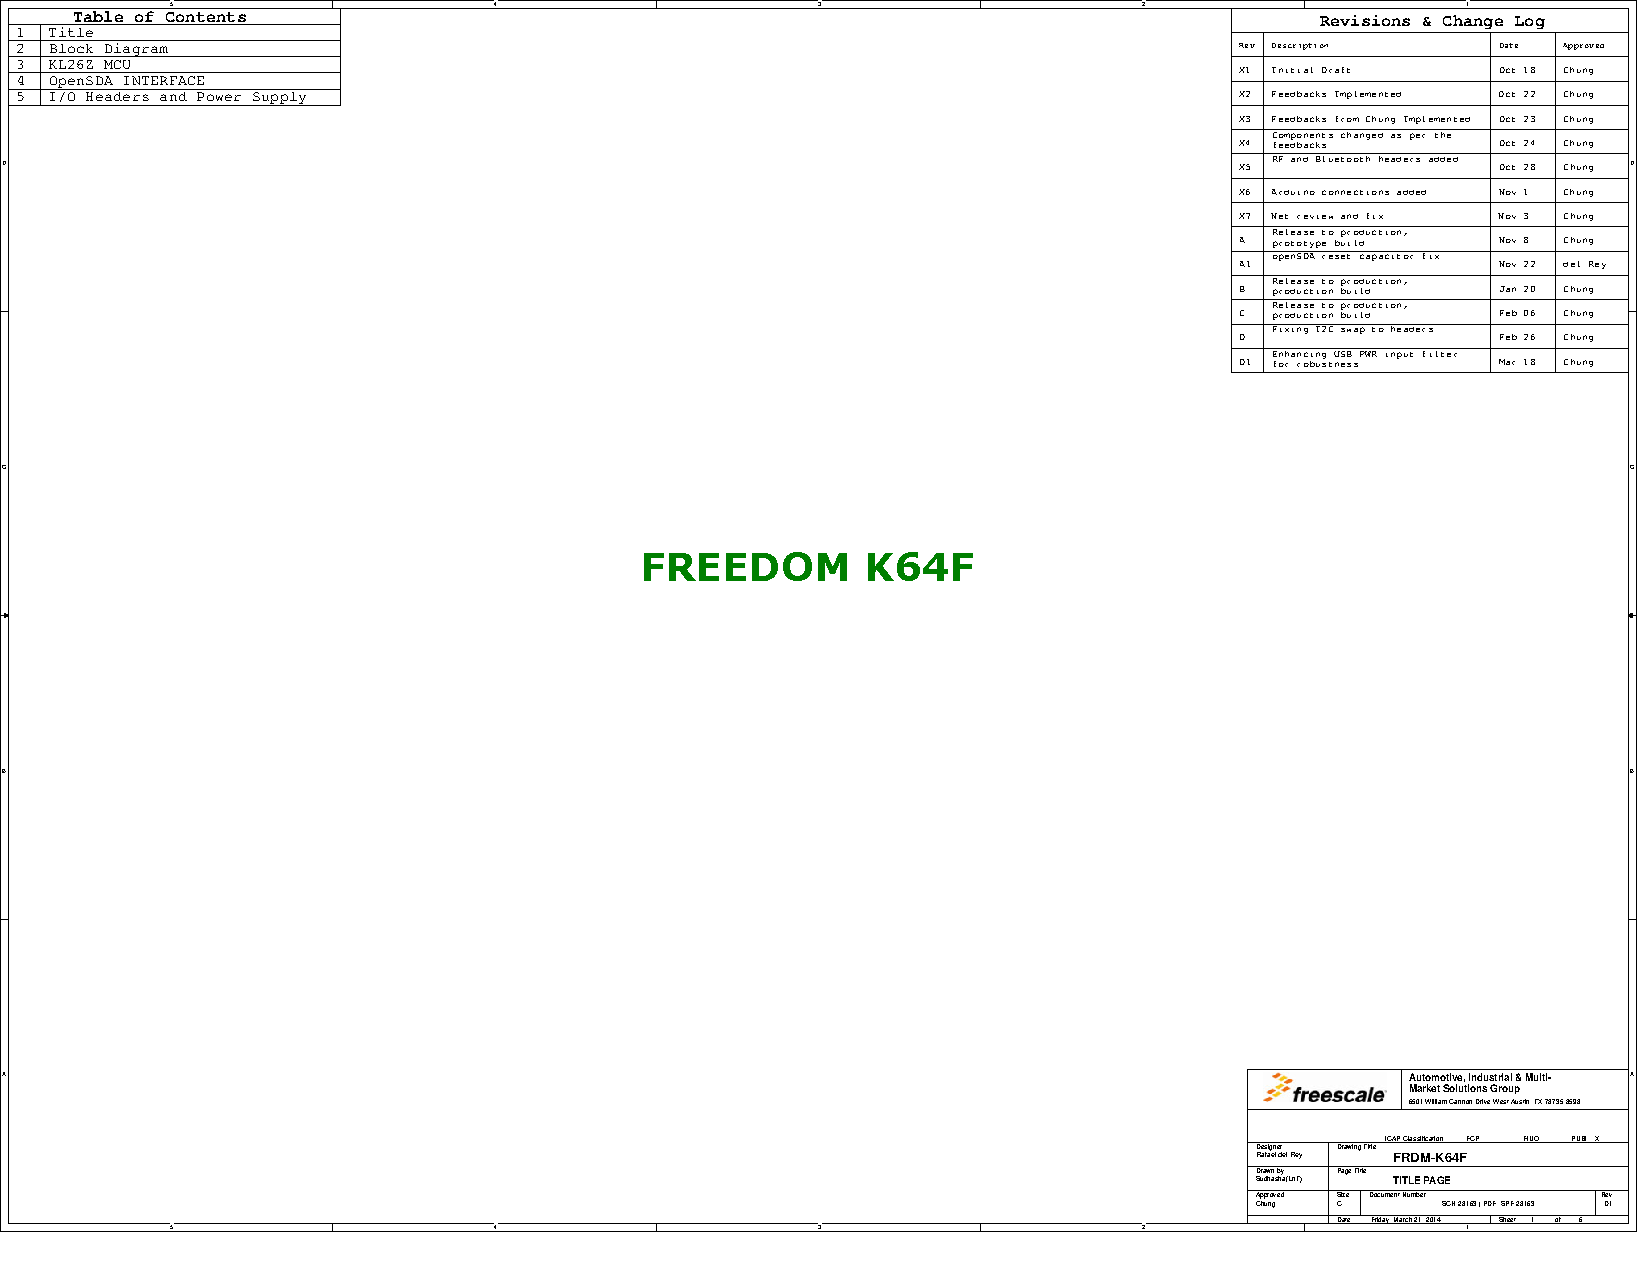
\includepdf[pages=-]{APPENDICES/k64fcircuitdiagram.pdf}
	\chapter{Ethics Form}
	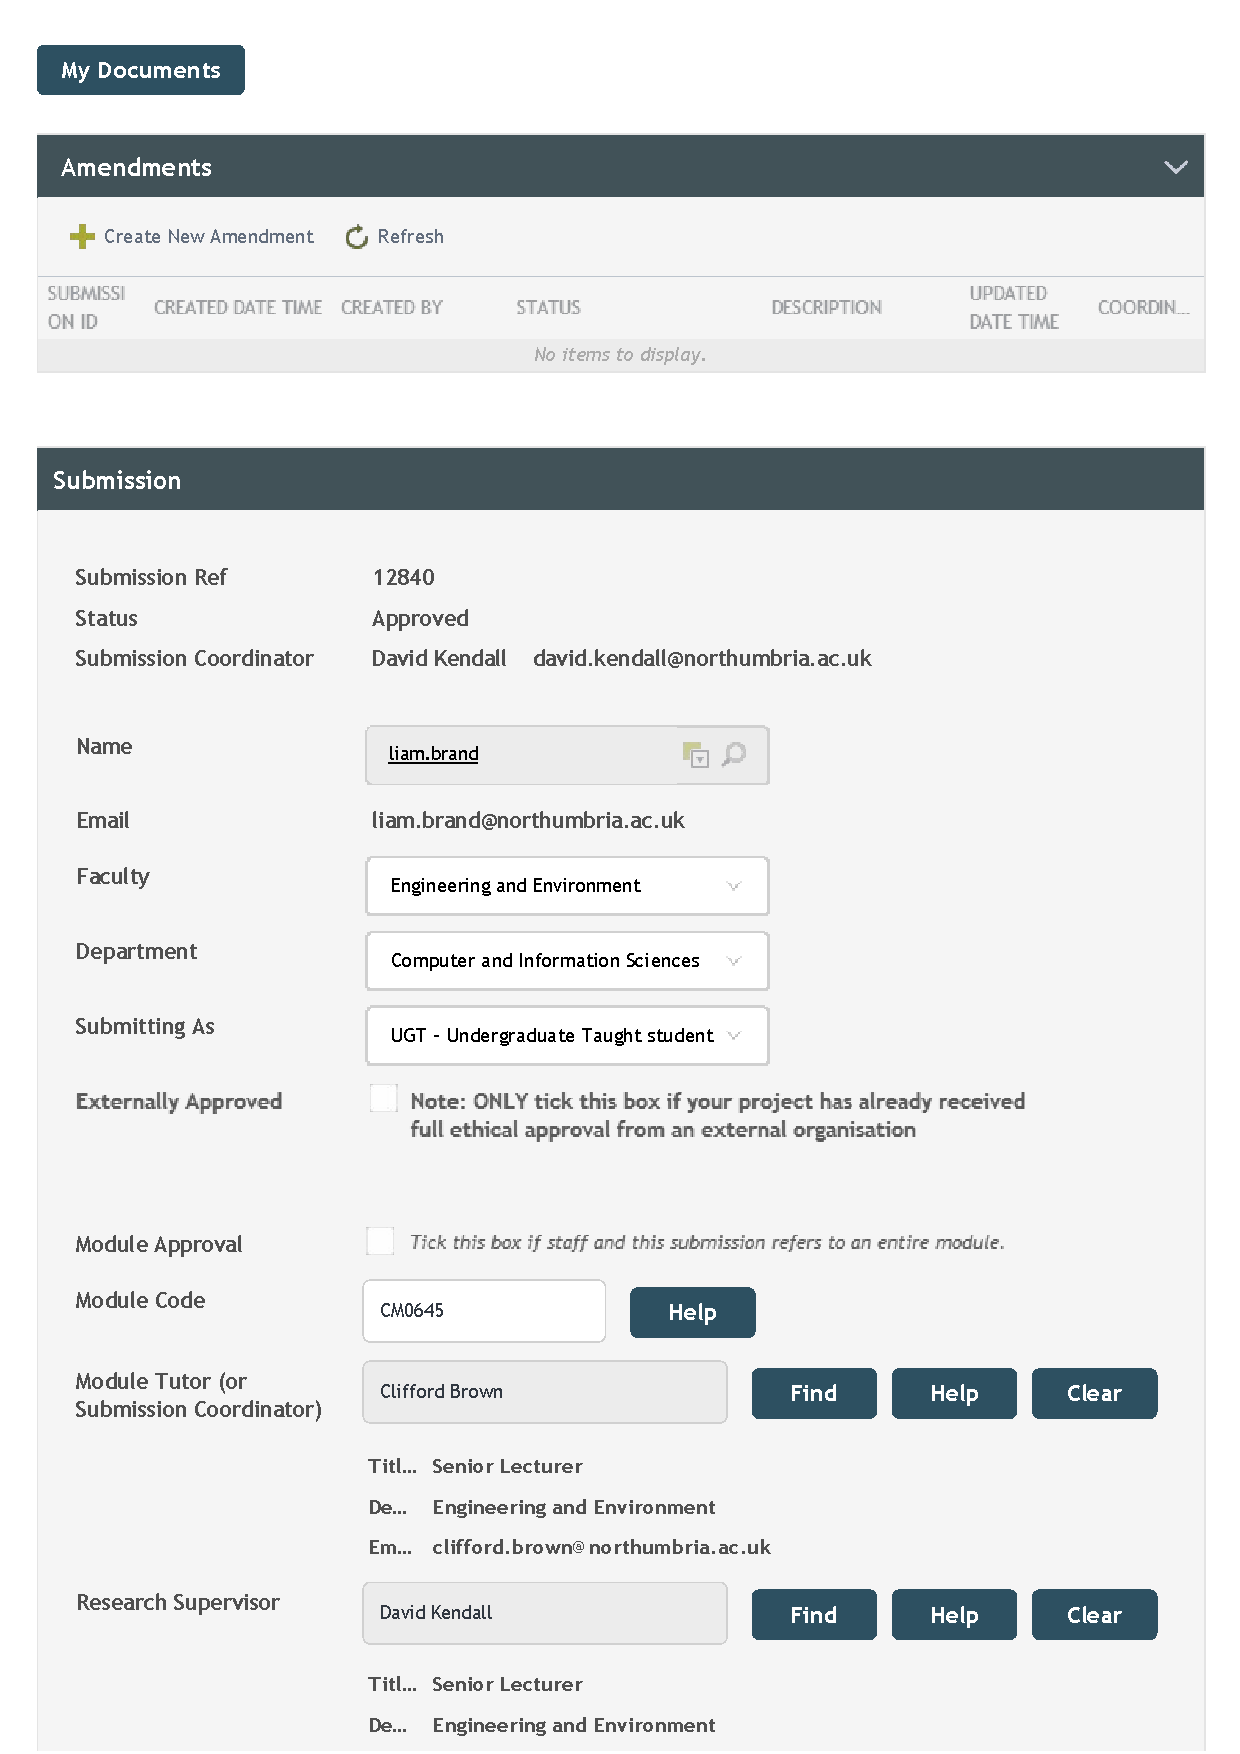
\includepdf[pages=-]{APPENDICES/ethicsonlineform.pdf}
	\end{appendices}
			

	% GLOSSARY -- include if you've used lots of technical terminology/notation
	% \include{glossary}
	\nocite{stachniss2013robotmappingintro}
	
\end{document}